% !TeX program = pdflatex
% =============================================================================
% Vorlage: Arbeitsblatt (nicht bewertet, Übungsmaterial für den Unterricht)
% Kantonsschule KFR – Physik
%
% Verwendung:
%   1. Diese Datei nach arbeitsblaetter/<klasse>/<semester>/<thema>/ kopieren
%      und sinnvoll umbenennen, z. B.
%      arbeitsblaetter/5-klasse/1-hs/thermodynamik/waermeleitung-arbeitsblatt.tex
%   2. \Klasse/\Thema/\ArbeitsblattTitel anpassen (weiter unten, vor
%      \begin{document}). \Datum füllt sich automatisch mit dem aktuellen
%      Datum (\today); Lehrperson ist fest auf "Loris Keller" gesetzt.
%      Kein Tabellenraster mehr -- Klasse/Datum/Thema/Lehrperson stehen als
%      einfache Textzeile unter dem Titel-Banner.
%   3. Jedes Arbeitsblatt beginnt mit einem Lernziele-Block (\begin{infobox})
%      direkt nach der Kopfzeile, noch vor der ersten Aufgabe -- Stichpunkte
%      pro Arbeitsblatt anpassen, den Block selbst nicht entfernen.
%   4. Direkt danach folgt IMMER ein Theorie-Block (\begin{theoriebox}) --
%      die fachliche Grundlage (Definitionen, Formeln, Merksätze), die für
%      die nachfolgenden Aufgaben gebraucht wird, in eigener grüner Box.
%      Reihenfolge im Dokument ist fest: Lernziele (blau) -> Theorie (grün)
%      -> Aufgaben (blau, taskbox). Theorie-Inhalt vor den Aufgaben
%      ausformulieren, nicht als Lückenfüller stehen lassen.
%   5. Aufgaben mit \question[Punktzahl] ... ergänzen, Lösung jeweils in
%      \begin{solution}...\end{solution} setzen. \begin{taskbox}...\end{taskbox}
%      ist optional und rahmt eine Aufgabe farbig ein.
%   6. Lösungen ein-/ausblenden: \printanswers (Lehrerexemplar) bzw.
%      \noprintanswers (Schülerexemplar, Standard) weiter unten umschalten.
% =============================================================================
\documentclass[addpoints,11pt,a4paper]{exam}

\usepackage[T1]{fontenc}
\usepackage[utf8]{inputenc}
\usepackage[ngerman]{babel}
\usepackage{lmodern}
\usepackage[a4paper,margin=2.2cm,headheight=14pt]{geometry}
\usepackage{amsmath}
\usepackage{siunitx}
% Hausstil: zusammengesetzte Einheiten immer als echter Bruch (\frac), nicht
% als Inline-Schrägstrich oder \tfrac -- gilt global für jedes \si/\SI.
\sisetup{per-mode=fraction,fraction-command=\frac}
\usepackage{array,booktabs,tabularx,multirow}
\usepackage{enumitem}
\usepackage{graphicx}
\usepackage{xcolor}
\usepackage{colortbl}
\usepackage{tikz}
\usepackage{physics}
\usepackage{circuitikz}
\usepackage[most]{tcolorbox}
\usepackage{lastpage}
\usepackage{needspace}

\usetikzlibrary{arrows.meta,calc,angles,quotes}

\usepackage{setspace}
\setlength{\parindent}{0pt}
\setlength{\parskip}{0.6em}
% Hausstil v2: etwas grosszügigerer Zeilenabstand als Standard-LaTeX (1.0),
% damit Fliesstext innerhalb der Boxen weniger gedrängt wirkt -- 1.08 ist
% bewusst dezent gewählt (nicht \onehalfspacing/1.5), um nicht unnötig
% Platz/Seiten zu kosten.
\setstretch{1.08}
% Etwas grosszügigerer Standardabstand zwischen Listenpunkten (gilt für
% jede \begin{itemize}, sofern nicht lokal überschrieben).
\setlist[itemize]{itemsep=0.4em}

% -----------------------------
% Farben (Corporate-Farbschema Physik KFR)
% -----------------------------
\definecolor{titleblue}{HTML}{183A6B}
\definecolor{accentblue}{HTML}{2E6F9E}
\definecolor{lightblue}{HTML}{EAF4FB}
\definecolor{verylightblue}{HTML}{F7FBFE}
\definecolor{lightgray}{HTML}{F4F6F8}
\definecolor{darkgray}{HTML}{4A4A4A}
% Für Diagramme mit zwei verschiedenen Funktionen/Linien: titleblue (dunkles
% Blau) + accentorange (Orange) sind weit genug auseinander (auch in
% Graustufen/für Farbenblinde unterscheidbar), im Gegensatz zu
% titleblue+accentblue, die beide Blautöne sind.
\definecolor{accentorange}{HTML}{D9720C}
% Für Diagramme mit DREI Linien (z.B. Bildfahrplan mit drei Zügen): dritte
% Farbe nötig, die sich sowohl von titleblue als auch von accentorange klar
% unterscheidet -- auch in Graustufen/für Farbenblinde. Violett liegt weit
% genug von Blau und Orange entfernt, um als dritte Linie eindeutig
% unterscheidbar zu bleiben.
\definecolor{accentpurple}{HTML}{7B2D8E}
% Theorie-Block: eigene Farbe (grün), damit er sich auf einen Blick von den
% blauen Lernziele-/Aufgaben-Boxen abhebt.
\definecolor{theorygreen}{HTML}{2E7D4F}
\definecolor{lighttheorygreen}{HTML}{EAF7EF}
% Gruppenarbeit-Box: eigene Farbe (Petrol/Teal), damit Partner-/Gruppenarbeit
% sich auf einen Blick von normalen Einzelaufgaben (blau, taskbox) und vom
% Theorie-Block (grün, theoriebox) abhebt. Siehe Regel weiter unten bei
% \newtcolorbox{groupbox}.
\definecolor{groupteal}{HTML}{1B7F72}
\definecolor{lightgroupteal}{HTML}{E8F5F3}

% -----------------------------
% Spaltentypen
% -----------------------------
\newcolumntype{Y}{>{\centering\arraybackslash}X}
\newcolumntype{P}[1]{>{\raggedright\arraybackslash}p{#1}}

% -----------------------------
% Boxen
% -----------------------------
% Hausstil v2: einheitlicher Abstand VOR/NACH jeder Box (Titelbox, Info-,
% Theorie-, Task-, Beispiel-, Gruppen-, Antwortbox), damit Boxen nicht
% direkt am umgebenden Fliesstext oder aneinander kleben. Als globale
% tcolorbox-Vorgabe gesetzt statt einzeln pro Box, damit sie für alle
% \newtcolorbox-Definitionen unten automatisch gilt.
\tcbset{before skip=10pt, after skip=10pt}
\newtcolorbox{titlebox}{
  enhanced,
  colback=titleblue,
  colframe=titleblue,
  boxrule=0pt,
  arc=3mm,
  left=3mm,right=3mm,top=3mm,bottom=3mm
}

% exam.cls rückt die questions-Liste um die Breite von "10." (plus \labelsep)
% ein (Platz für die Nummerierung "1.", "2." ...); wir messen dieselbe Distanz
% hier unabhängig nach.
\newlength{\aufgabenindent}
\settowidth{\aufgabenindent}{10.\hskip\labelsep}

% left/right-Padding bewusst grosszügiger als bei answerbox: exam.cls hängt
% die Nummerierung von \question bündig an den inneren Rand des
% Textbereichs -- bei zu knappem Padding sitzt diese Nummer direkt auf dem
% Rahmen der Box statt sichtbar innerhalb davon.
% infobox steht ausserhalb von questions (z.B. beim Lernziele-Block auf
% Dokumentebene) und braucht deshalb KEINE Korrektur -- \linewidth entspricht
% dort bereits \textwidth.
\newtcolorbox{infobox}{
  enhanced,
  breakable,
  colback=lightblue,
  colframe=accentblue,
  boxrule=0.7pt,
  arc=2mm,
  left=6mm,right=6mm,top=3.5mm,bottom=3.5mm
}

% theoriebox: wie infobox, aber grün und mit farbigem Titelbalken (analog zu
% taskbox), damit der Theorie-Block auf einen Blick von Lernziele (blau,
% ohne Titelbalken) und Aufgaben (blau, mit Titelbalken) unterscheidbar ist.
% Steht wie infobox ausserhalb von questions -- KEINE Einrückungskorrektur
% nötig (siehe Kommentar bei infobox oben).
% Regel: hervorgehobene/definierte Begriffe INNERHALB einer theoriebox
% immer mit \textbf{\emph{...}} setzen (fett UND kursiv), nicht mit blossem
% \emph{...} -- damit Fachbegriffe beim Durchlesen der Theorie sofort
% auffallen. Ausserhalb von theoriebox (beispielbox, Aufgabentext, ...)
% bleibt \emph{...} allein korrekt.
\newtcolorbox{theoriebox}[1][Theorie]{
  enhanced,
  breakable,
  colback=lighttheorygreen,
  colframe=theorygreen,
  title={#1},
  fonttitle=\bfseries,
  boxrule=0.7pt,
  arc=2mm,
  left=6mm,right=6mm,top=3.5mm,bottom=3.5mm
}

% taskbox steht direkt in der questions-Liste (vor dem ersten \question),
% also innerhalb von deren Einrückung. Empirisch (per Pixelvergleich mit der
% Kopfzeilen-Tabelle) verschiebt "enlarge left by" hier die GESAMTE Box
% (nicht nur ihren linken Rand) -- ein positiver Wert schiebt sie nach
% RECHTS, nicht nach links, entgegen der naheliegenden Lesart des
% Schlüsselnamens. Ein negativer Wert (-\aufgabenindent) schiebt die Box
% exakt um die Listen-Einrückung nach links; width=\textwidth stellt danach
% wieder die volle Breite her, sodass beide Kanten mit der Tabelle
% übereinstimmen (verifiziert per Pixelmessung, Abweichung <=1px @300dpi).
% Falls taskbox künftig auch ausserhalb von questions verwendet wird, muss
% diese Korrektur analog zu infobox entfernt werden.
\newtcolorbox{taskbox}[1][]{
  enhanced,
  breakable,
  colback=verylightblue,
  colframe=accentblue,
  title={#1},
  fonttitle=\bfseries,
  boxrule=0.7pt,
  arc=2mm,
  enlarge left by=-\aufgabenindent,
  width=\textwidth,
  left=6mm,right=6mm,top=3.5mm,bottom=3.5mm
}

% beispielbox: wie taskbox (blau), aber ausserhalb von questions -- deshalb
% wie infobox/theoriebox KEINE Einrückungskorrektur nötig (siehe Kommentar
% bei infobox oben). Für Beispiele in der Theorie: farblich blau wie
% Aufgaben, damit "Beispiel" sich auf einen Blick von der grünen Theorie
% abhebt (Hausstil: grün = Theorie, blau = Beispiele/Aufgaben).
\newtcolorbox{beispielbox}[1][Beispiel]{
  enhanced,
  breakable,
  colback=verylightblue,
  colframe=accentblue,
  title={#1},
  fonttitle=\bfseries,
  boxrule=0.7pt,
  arc=2mm,
  left=6mm,right=6mm,top=3.5mm,bottom=3.5mm
}

% groupbox: Regel -- JEDE Aufgabe, bei der Schülerinnen/Schüler zu zweit
% oder in einer Gruppe zusammenarbeiten (Partnerarbeit, Gruppenarbeit,
% Diskussion zu zweit, ...), bekommt diese Box statt der blauen taskbox.
% Farbe (Petrol/Teal) ist bewusst weder blau (taskbox/infobox) noch grün
% (theoriebox), damit "hier braucht es eine Partnerin/einen Partner" auf
% einen Blick erkennbar ist. Strukturell identisch zu taskbox (gleiche
% Einrückungskorrektur, da auch groupbox innerhalb von questions steht).
\newtcolorbox{groupbox}[1][Gruppenarbeit]{
  enhanced,
  breakable,
  colback=lightgroupteal,
  colframe=groupteal,
  title={#1},
  fonttitle=\bfseries,
  boxrule=0.7pt,
  arc=2mm,
  enlarge left by=-\aufgabenindent,
  width=\textwidth,
  left=6mm,right=6mm,top=3.5mm,bottom=3.5mm
}

\newtcolorbox{answerbox}{
  breakable,
  colback=white,
  colframe=gray!55,
  boxrule=0.5pt,
  arc=1.5mm,
  left=2mm,right=2mm,top=2mm,bottom=2mm
}

% --- Lösungen ein-/ausblenden -----------------------------------------------
% Schülerexemplar (Standard): \noprintanswers
% Lehrer-/Lösungsexemplar:    \printanswers
\noprintanswers
%\printanswers

% --- Punkte bleiben intern, werden aber nicht gedruckt ----------------------
% Arbeitsblätter sind nicht benotet. \question[n]/\part[n] bekommen trotzdem
% eine Punktzahl n -- rein als interner Anhaltspunkt, der 1:1 an
% \Antwortraum{n} weitergereicht wird, um die Antwortraum-Grösse zu
% bestimmen. \pointformat{} (Aufruf, nicht \renewcommand!) unterdrückt die
% von der exam-Klasse sonst automatisch gedruckte Punktanzeige ("(n P.)")
% vollständig, ohne die interne Punktezählung (\numpoints) zu beeinflussen.
\pointformat{}

% --- Lösungsbox auf Deutsch, farblich abgesetzt -----------------------------
\renewcommand{\solutiontitle}{\noindent\color{titleblue}\textbf{Lösung:}\enspace}

% --- Kopf-/Fusszeile: Thema/Titel oben, Seitenzahl unten --------------------
\pagestyle{headandfoot}
\cfoot{\textcolor{darkgray}{Seite \thepage\ von \pageref{LastPage}}}

% --- Kopfzeile: Klasse / Datum / Thema / Titel ------------------------------
% Einheitliches Layout für Arbeitsblatt, Prüfung und Praktikum. Ohne Tabelle:
% Klasse/Datum/Thema/Lehrperson stehen als einfache Textzeile unter dem
% Titel-Banner.
\newcommand{\Kopfzeile}[4]{%
  \begin{titlebox}
    {\color{white}\sffamily\bfseries\Large #4}
  \end{titlebox}
  \noindent\textbf{Klasse:}~#1 \hfill \textbf{Datum:}~#2 \hfill \textbf{Thema:}~#3
    \hfill \textbf{Lehrperson:}~Loris Keller
  \lhead{\textcolor{darkgray}{#3}}
  \rhead{\textcolor{darkgray}{#4}}
}

% --- Antwortraum: ca. 2.5 cm Platz pro Punkt, als umrandetes Feld -----------
\newlength{\antwortraumlen}
\newcommand{\Antwortraum}[1]{%
  \pgfmathsetlength{\antwortraumlen}{#1*2.5cm}%
  \begin{answerbox}
    \rule{0pt}{\antwortraumlen}%
  \end{answerbox}%
}

% Werte für Kopfzeile zentral setzen
\newcommand{\Klasse}{4a}
\newcommand{\Datum}{21.08.2026}
\newcommand{\Thema}{s-t-Diagramm}
\newcommand{\ArbeitsblattTitel}{Arbeitsblatt: s-t-Diagramm}

\begin{document}

\Kopfzeile{\Klasse}{\Datum}{\Thema}{\ArbeitsblattTitel}

% --- Lernziele: aus lernziele.md (Backward-Design, Stufe 1) übernommen,
% aber NEU NUMMERIERT -- LZ1..LZ9 hier entsprechen der Reihenfolge, in der
% die zugehörigen Theorieboxen/Übungen im Dokument erscheinen (LZ1 = das
% im Arbeitsblatt zuerst behandelte Lernziel), NICHT der ursprünglichen
% Nummerierung aus dem Backward-Design-Dokument. lernziele.md wurde
% entsprechend mitnummeriert (und LZ1 inhaltlich verengt, siehe unten) --
% bei künftigen inhaltlichen Änderungen dort UND im Backward-Design-
% Dokument anpassen, nicht nur hier.
% LZ1 wurde bewusst verengt auf "was ist eine gleichförmige Bewegung, wie
% sieht ihr s-t-Diagramm aus" (Theoriebox "Lineare Bewegung: Geschwindigkeit
% als Steigung", die den Begriff "gleichförmige Bewegung" jetzt explizit
% nennt) -- NICHT mehr die volle Ruhe/gleichförmig/ungleichförmig-
% Klassifikation. Diese bleibt als Inhalt in der Theoriebox "Bewegungs-
% abschnitte im kombinierten Diagramm" erhalten, aber ohne eigene LZ-Nummer
% (reine Vertiefung, analog zu "Einheiten umrechnen"/"Der Betrag einer Zahl").
% Reihenfolge: LZ1 (Weg vs. Ortsänderung) -> LZ2 (Zeit läuft nur vorwärts)
% -> LZ3 (gleichförmige Bewegung: Definition + Diagrammform) -> LZ4
% (Durchschnittsgeschwindigkeit als Sekante) -> LZ5 (drei Grundbewegungen,
% Vorzeichen der Steigung) -> LZ6/LZ7 (Partnerarbeit Bewegungsgeschichte --
% keine eigene Theoriebox, daher nach deren Übungsposition eingeordnet) ->
% LZ8/LZ9 (Momentangeschwindigkeit/Tangente, Grenzwert-Definition). Bei
% künftigen inhaltlichen Ergänzungen diese Reihenfolge mit anpassen.
\begin{infobox}
\textbf{Lernziele}\\
Am Ende dieser Einheit kann ich \dots
\begin{itemize}[leftmargin=1.2cm,itemsep=0.4em]
  \item anhand eines s-t-Diagramms mit Richtungswechsel den Unterschied zwischen zurückgelegtem Weg und Ortsänderung erklären. (LZ1)
  \item begründen, weshalb eine vertikale Linie im s-t-Diagramm physikalisch nicht möglich ist. (LZ2)
  \item erklären, was eine gleichförmige Bewegung ist, und wie das zugehörige s-t-Diagramm aussieht. (LZ3)
  \item zu zwei Zeitpunkten $t_1$, $t_2$ die Durchschnittsgeschwindigkeit $\bar v = \Delta s/\Delta t$ als Sekantensteigung berechnen. (LZ4)
  \item positive, negative und verschwindende Steigungen den Bewegungsrichtungen vorwärts/rückwärts/Stillstand zuordnen. (LZ5)
  \item zu einer Bewegungsbeschreibung ein passendes s-t-Diagramm skizzieren. (LZ6)
  \item ein s-t-Diagramm ohne weitere Angaben in eigenen Worten so beschreiben, dass eine fachfremde Person die Bewegung versteht. (LZ7)
  \item an einem markierten Punkt die Tangente einzeichnen und die Momentangeschwindigkeit qualitativ abschätzen. (LZ8)
  \item erklären, weshalb die Momentangeschwindigkeit der Grenzwert der Durchschnittsgeschwindigkeit für $\Delta t \to 0$ ist. (LZ9)
\end{itemize}
\end{infobox}

% --- Einstieg: Hook vor der formalen Theorie, Bilder aus Bilder/ -----------
\begin{beispielbox}[Einstieg: Woher weiss die SBB, wann der Zug kommt?]
Ihr wartet auf einen Zug. Woher weiss die SBB, dass er um 14:32 hier
ankommt und nicht um 14:28 oder 14:40? Und woher weiss die App, wo der Zug
gerade ungefähr ist, obwohl kein GPS-Sender ständig meldet?

% Lehrperson: Hier kurz innehalten und die Klasse raten lassen, bevor die
% beiden Bilder unten gezeigt/besprochen werden. Keine Auflösung im
% Dokument -- die Vermutungen sollen im Gespräch entstehen.

\medskip
\begin{center}
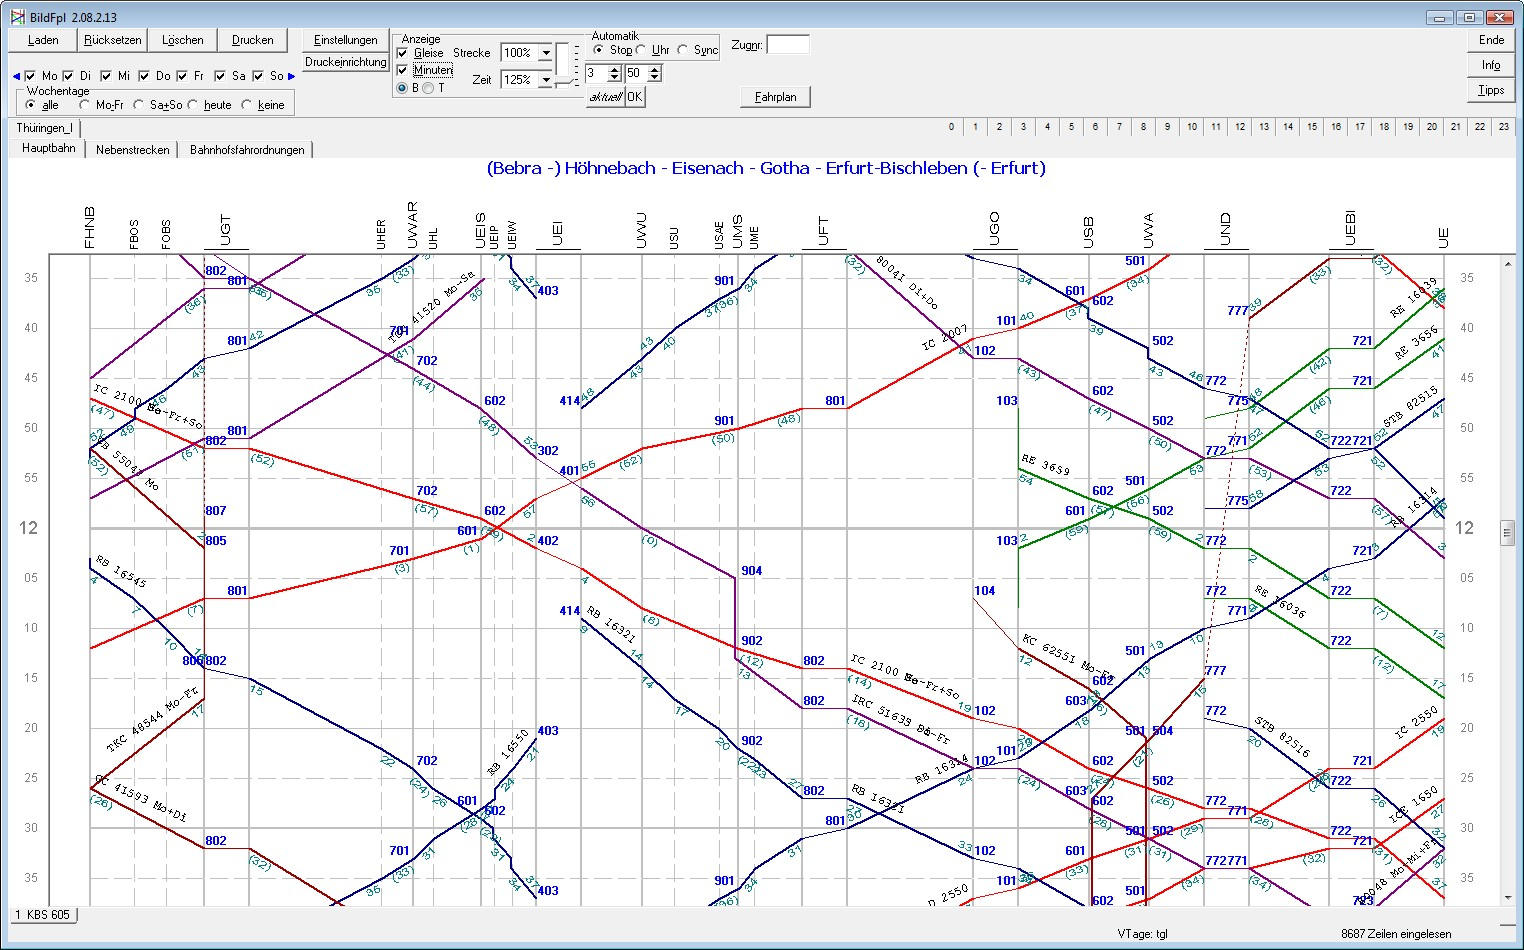
\includegraphics[width=0.75\linewidth]{Bilder/Bildfahrplan.jpg}\\
\footnotesize Bildfahrplan einer Bahnstrecke (Beispiel): jede farbige Linie ist ein Zug.
\end{center}

So planen Bahnbetriebe (darunter auch die SBB) ihre Fahrpläne: in
einem sogenannten \emph{Bildfahrplan}. Die waagrechte Achse zeigt die
Zeit, die senkrechte Achse die Position entlang der Strecke. Jede farbige
Linie ist ein einzelner Zug. Die \emph{Steigung} einer Linie ist genau
das, was wir in diesem Arbeitsblatt als Geschwindigkeit $v=\Delta
s/\Delta t$ kennenlernen werden: Je steiler eine Linie, desto schneller
der Zug. Eine \emph{waagrechte} Linie bedeutet, dass ein Zug an einem
Bahnhof steht (Geschwindigkeit $=0$). Und wo sich zwei Linien
\emph{kreuzen}, befinden sich zwei Züge zur gleichen Zeit am gleichen
Ort. Deshalb werden solche Kreuzungspunkte bei der Fahrplanung extrem
genau berechnet.

\medskip
\begin{center}
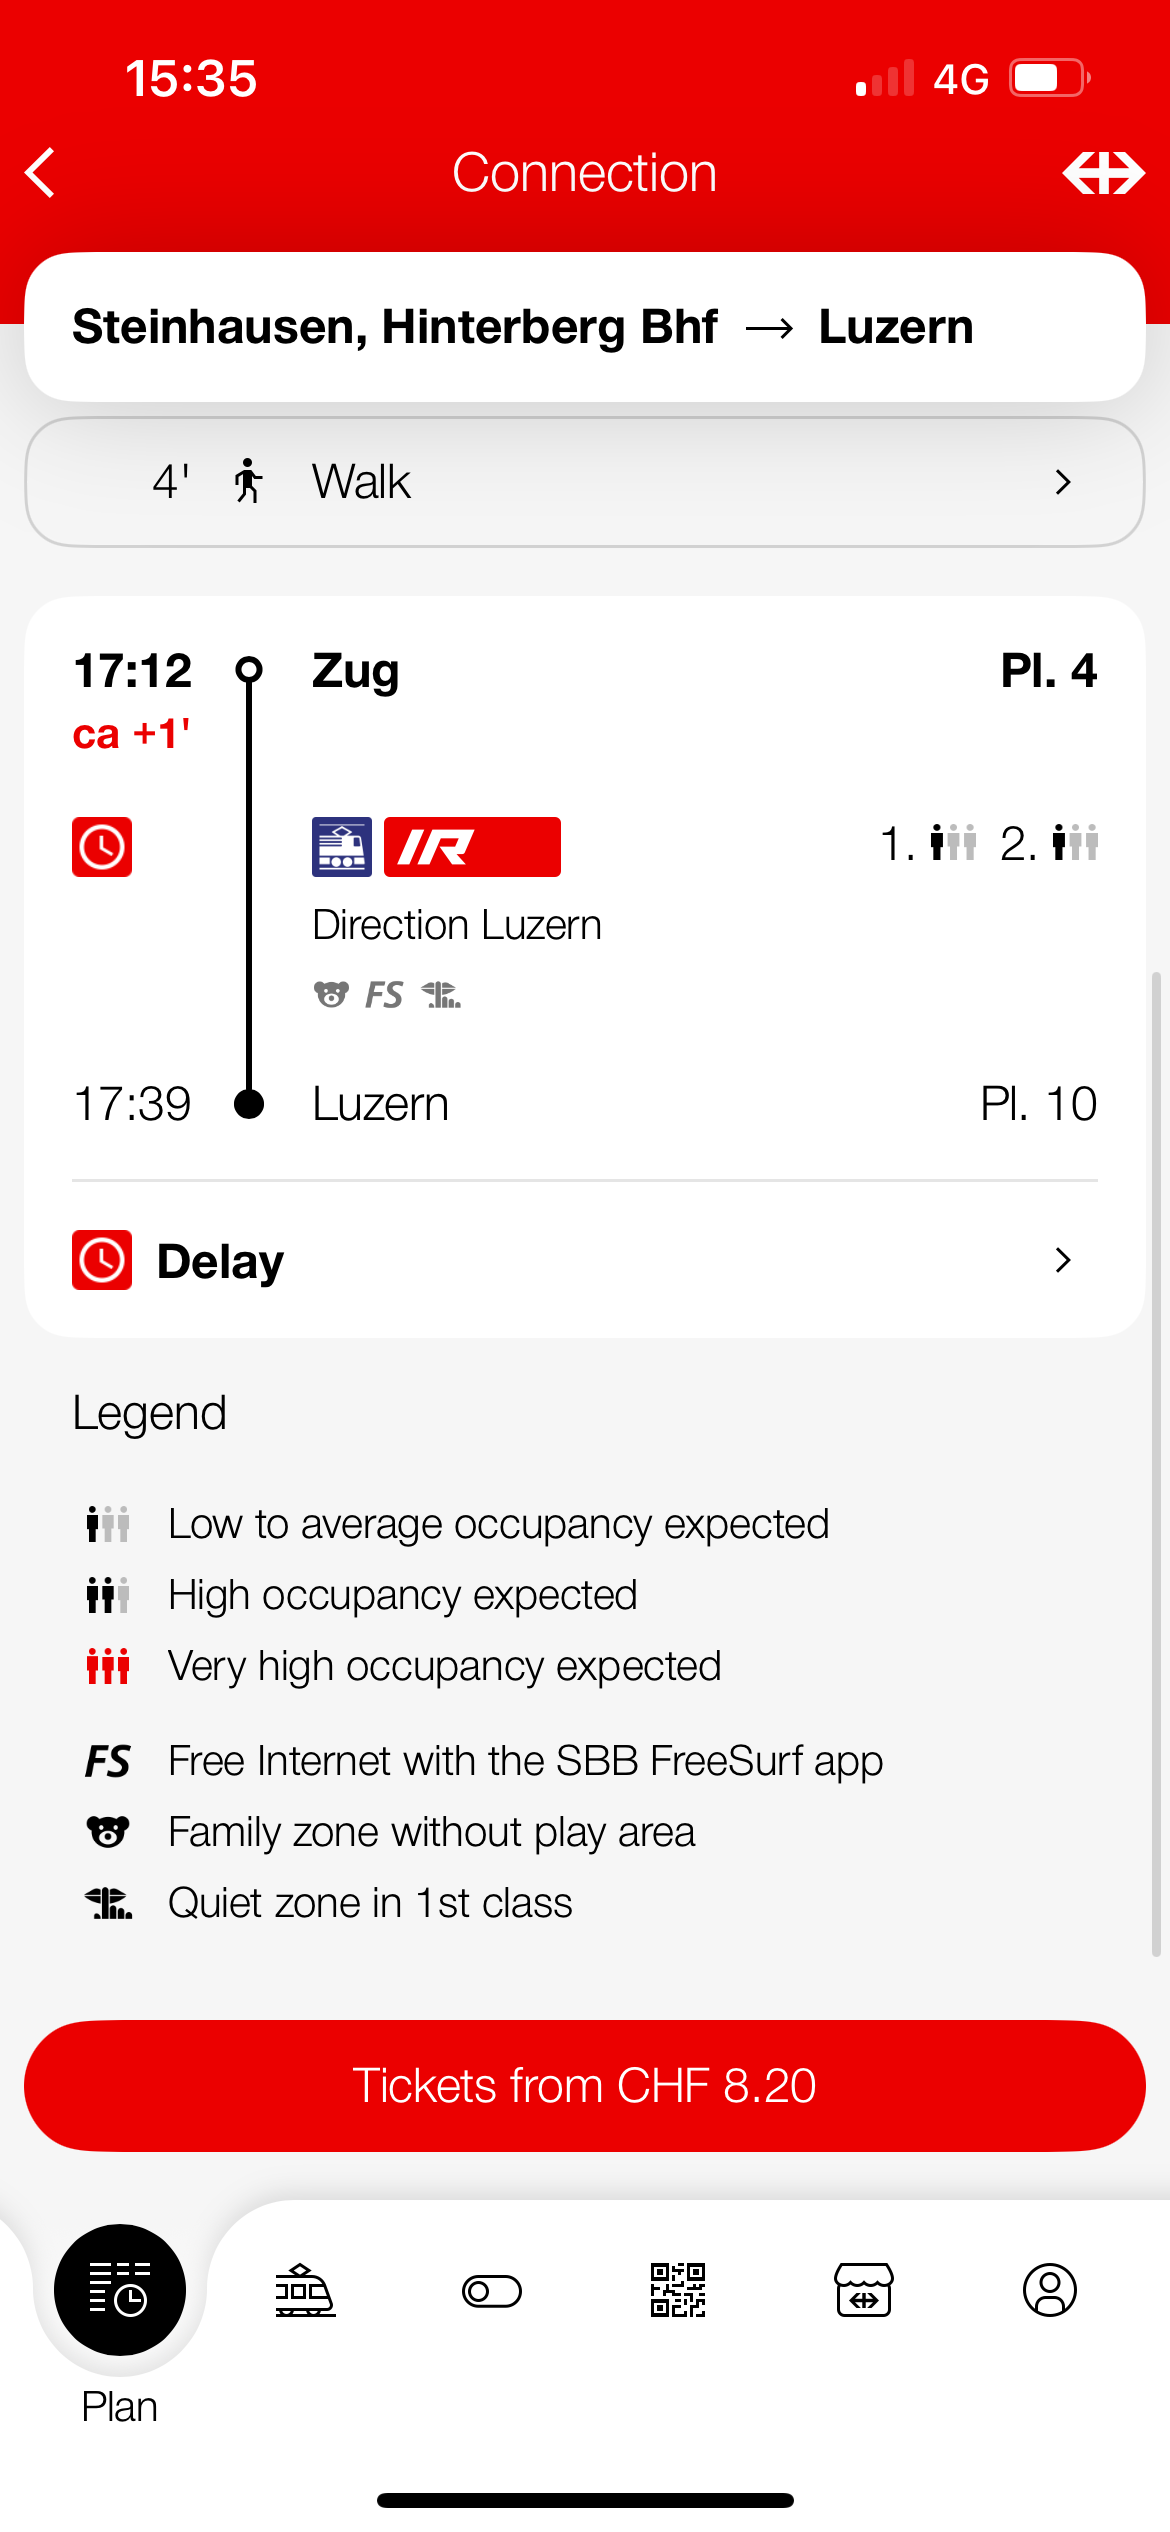
\includegraphics[width=0.26\linewidth]{Bilder/SBB_app.png}\\
\footnotesize SBB-App: geplante Zeit (Soll) und Verspätung (Ist $-$ Soll).
\end{center}

Genau diese Logik steckt auch hinter der SBB-App. Die Position eines
Zuges zeigt sie nicht per ununterbrochenem Live-GPS an, sondern rechnet
sie oft schlicht \emph{hoch}: aus der letzten bekannten Abfahrtszeit
$t_0$ an einer Haltestelle (Ort $s_0$) und der bekannten Geschwindigkeit
$v$ des Zuges ergibt sich die aktuelle Position als
\[
  s = s_0 + v\cdot(t-t_0),
\]
also genau die Formel, die wir in dieser Lektion herleiten werden. Auch
eine \emph{Verspätung}, wie im Screenshot oben (\glqq ca.\,+1'\grqq{})
angezeigt, ist nichts anderes als eine Zeitdifferenz: der Unterschied
zwischen der geplanten Zeit (Soll) und der tatsächlich beobachteten Zeit
(Ist).

Genau um solche Fragen geht es in diesem Arbeitsblatt: Wie berechnet man
aus einem Diagramm Geschwindigkeiten, Positionen und Zeitdifferenzen? Wir
beginnen mit dem einfachsten Fall: dem $s$-$t$-Diagramm.
\end{beispielbox}

% --- Theorie: fachliche Grundlage für die Aufgaben 1--4, in eigene Boxen
%     unterteilt (je Unterthema eine theoriebox) --------------------------
\begin{theoriebox}[Das s-t-Diagramm: Ort als Funktion der Zeit]
Der \textbf{\emph{Ort}} $s$ eines Objekts ist eine Koordinate auf einer festgelegten,
eindimensionalen Bewegungsachse: Man legt einen Nullpunkt ($s=0$) und eine
positive Richtung fest. Jedem Ort entspricht genau eine Zahl $s$ in
$\si{\meter}$ (positiv, negativ oder null).

Die \textbf{\emph{Zeit}} $t$ (Einheit: $\si{\second}$) wird ab einem
Startzeitpunkt ($t=0$, meist der Beginn der Beobachtung) gemessen.

Ein \textbf{\emph{$s$-$t$-Diagramm}} trägt den Ort $s$ auf der senkrechten Achse
gegen die Zeit $t$ auf der waagrechten Achse auf. Jeder Punkt $(t,\,s(t))$
des Graphen beantwortet die Frage: \textbf{\emph{Wo befand sich das Objekt zum
Zeitpunkt $t$?}}

\begin{center}
\begin{tikzpicture}[scale=1.0]
  \draw[->] (-0.3,0) -- (6.3,0) node[right] {\scriptsize $s$ in m};
  \foreach \x in {0,1,2,3,4,5,6} \draw (\x,0.08) -- (\x,-0.08);
  \node[below] at (0,-0.25) {\scriptsize $0$};
  \filldraw[accentblue] (4.5,0) circle (2pt) node[above] {\scriptsize Ort $s=4.5\,$m};
\end{tikzpicture}

\begin{tikzpicture}[scale=0.85]
  \draw[gray!20] (0,0) grid (4,3);
  \draw[->] (-0.3,0) -- (4.7,0) node[right] {\scriptsize $t$ in s};
  \draw[->] (0,-0.3) -- (0,3.7) node[above] {\scriptsize $s$ in m};
  \foreach \x in {1,2,3,4} \draw (\x,0.06) -- (\x,-0.06) node[below] {\scriptsize \x};
  \foreach \y in {1,2,3} \draw (0.06,\y) -- (-0.06,\y) node[left] {\scriptsize \y};
  \draw[thick,titleblue] (0,1) -- (4,3);
  \draw[dashed,gray] (2,0) -- (2,2) -- (0,2);
  \filldraw[accentblue] (2,2) circle (1.6pt) node[above left,xshift=-1mm,yshift=2mm] {\scriptsize $(t,\,s(t))=(\SI{2}{\second},\,\SI{2}{\meter})$};
\end{tikzpicture}
\end{center}
\end{theoriebox}

\begin{beispielbox}[Beispiel: Auto auf der Autobahn]
\begin{minipage}[t]{0.6\linewidth}
Ein Auto befindet sich auf einer Autobahn bei der Kilometermarkierung
$s=\SI{2.6}{\kilo\meter}$ (gemessen ab einem festen Nullpunkt der
Autobahn, angezeigt durch einen Kilometerstein am Strassenrand, siehe
Foto). Ab diesem Zeitpunkt ($t=\SI{0}{\minute}$) fährt es in Richtung
steigender Kilometermarkierungen. Nach $t=\SI{15}{\minute}$ befindet es
sich bei $s=\SI{32.6}{\kilo\meter}$.
\end{minipage}%
\hfill
\begin{minipage}[t]{0.35\linewidth}
\centering
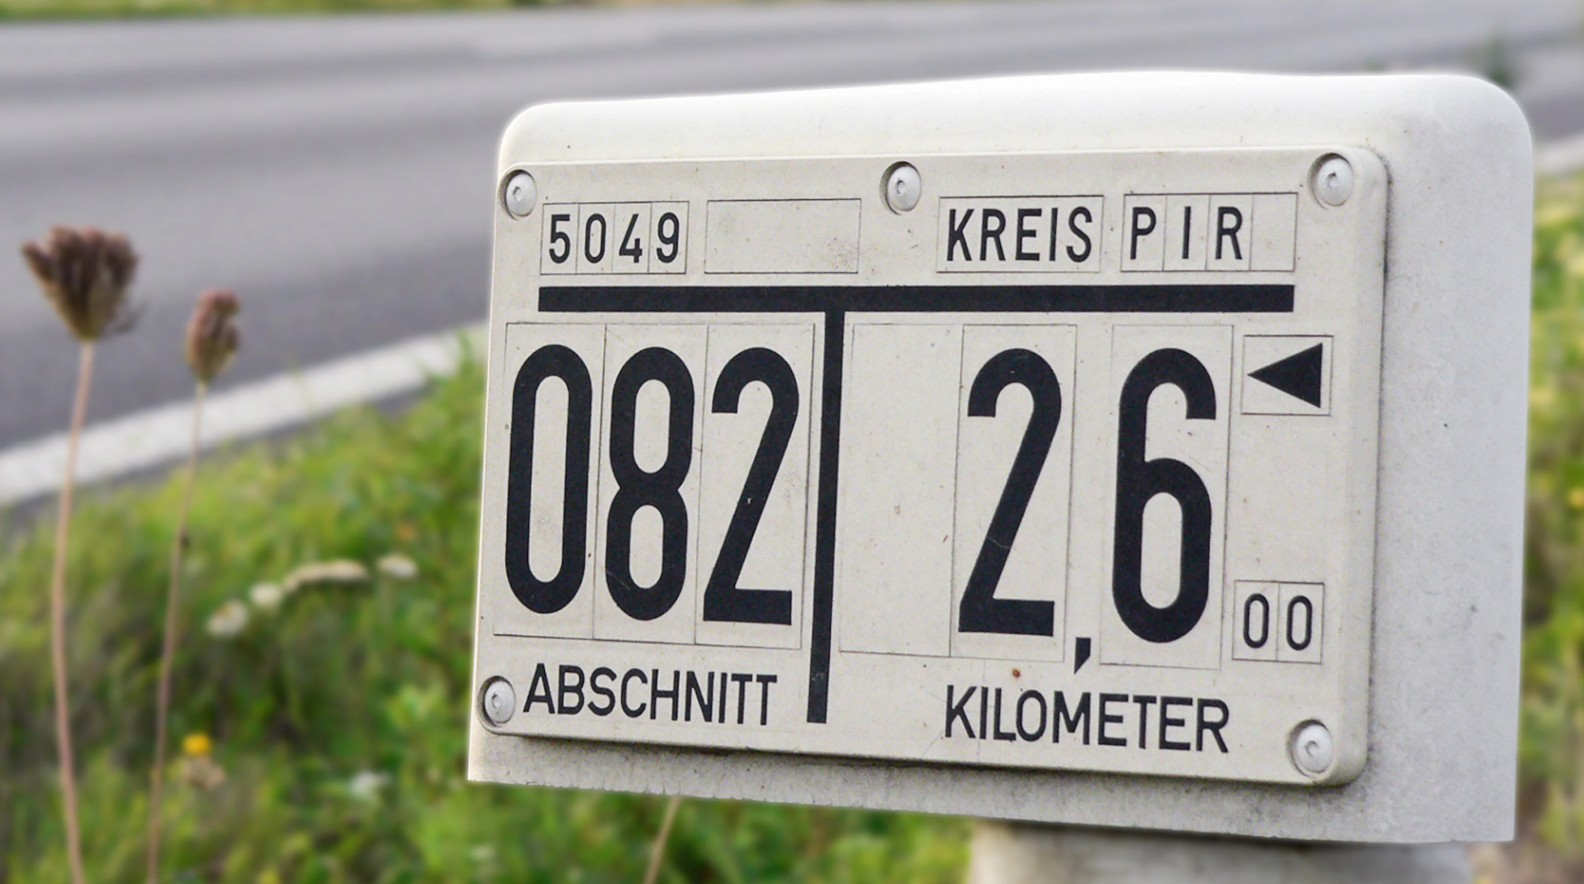
\includegraphics[width=0.8\linewidth]{Bilder/Kilometerstein.jpg}\\
\footnotesize Kilometerstein an einer Autobahn
\end{minipage}

\begin{center}
\begin{tikzpicture}[scale=1.0]
  \draw[gray!20] (0,0) grid (5,3);
  \draw[->] (-0.3,0) -- (5.7,0) node[right] {\scriptsize $t$ in min};
  \draw[->] (0,-0.3) -- (0,3.7) node[above] {\scriptsize $s$ in km};
  \foreach \x/\lbl in {1/3,2/6,3/9,4/12,5/15} \draw (\x,0.06) -- (\x,-0.06) node[below] {\scriptsize \lbl};
  \foreach \y/\lbl in {0/2.6,1/12.6,2/22.6,3/32.6} \draw (0.06,\y) -- (-0.06,\y) node[left] {\scriptsize \lbl};
  \draw[thick,titleblue] (0,0) -- (5,3);
  \filldraw[accentblue] (0,0) circle (1.6pt);
  \filldraw[accentblue] (5,3) circle (1.6pt);
\end{tikzpicture}

\footnotesize Start ($t=\SI{0}{\minute}$): $s=\SI{2.6}{\kilo\meter}$. \quad Ende ($t=\SI{15}{\minute}$): $s=\SI{32.6}{\kilo\meter}$.
\end{center}
\end{beispielbox}

\begin{theoriebox}[Zurückgelegter Weg vs.\ Ortsänderung]
Wechselt ein Objekt die Bewegungsrichtung, muss zwischen zwei Grössen
unterschieden werden: der \textbf{\emph{zurückgelegte Weg}} ist die Summe der
Beträge aller Teilstrecken (immer $\geq 0$), während die
\textbf{\emph{Ortsänderung}} nur den Unterschied zwischen End- und Anfangsposition
angibt ($s(t_2) - s(t_1)$, kann auch $0$ oder negativ sein). Bei einer
Bewegung ohne Richtungswechsel sind beide Werte gleich gross.

Die beiden folgenden Bewegungen zeigen das besonders deutlich: Beide
starten zur gleichen Zeit am gleichen Ort und befinden sich auch zur
gleichen späteren Zeit wieder am gleichen Ort. Die \textbf{\emph{Ortsänderung}}
ist also für beide identisch, trotzdem ist der \textbf{\emph{zurückgelegte Weg}}
nicht gleich gross.

\begin{center}
\begin{tikzpicture}[scale=0.55]
  \draw[gray!20] (0,0) grid[xstep=2,ystep=5] (10,15);
  \draw[->] (-0.3,0) -- (11.3,0) node[right] {\scriptsize $t$ in s};
  \draw[->] (0,-0.3) -- (0,16.5) node[above] {\scriptsize $s$ in m};
  \foreach \x in {2,4,6,8,10} \draw (\x,0.15) -- (\x,-0.15) node[below] {\scriptsize \x};
  \foreach \y in {5,10,15} \draw (0.15,\y) -- (-0.15,\y) node[left] {\scriptsize \y};
  \draw[thick,accentorange] (0,0) -- (10,10);
  \draw[thick,titleblue] (0,0) -- (5,15) -- (10,10);
  \filldraw[black] (0,0) circle (1.8pt);
  \filldraw[black] (10,10) circle (1.8pt);
\end{tikzpicture}

\footnotesize \textcolor{accentorange}{direkter Weg}: Weg $=\SI{10}{\meter}=$ Ortsänderung. \quad \textcolor{titleblue}{Umweg über $s=\SI{15}{\meter}$}: Weg $=\SI{15}{\meter}+\SI{5}{\meter}=\SI{20}{\meter}=2\times$ Ortsänderung.
\end{center}
\end{theoriebox}

\begin{questions}
\begin{taskbox}[Übung: Weg vs. Ortsänderung]
\question[4] Eine Velofahrerin trainiert auf einer geraden Uferstrasse
entlang eines Sees. Der Nullpunkt ($s=0$) markiert das Bootshaus in der
Mitte der Strecke; die positive Richtung zeigt nach Osten. Sie startet
$\SI{6}{\kilo\meter}$ westlich des Bootshauses (also bei
$s=-\SI{6}{\kilo\meter}$) und fährt nach Osten, bis sie bei
$t=\SI{27}{\minute}$ einen Aussichtspunkt $\SI{3}{\kilo\meter}$ östlich
des Bootshauses erreicht ($s=\SI{3}{\kilo\meter}$). Dort legt sie eine
$\SI{6}{\minute}$ lange Pause ein. Anschliessend kehrt sie um und fährt
nach Westen zurück, bis sie bei $t=\SI{51}{\minute}$ bei
$s=-\SI{4.5}{\kilo\meter}$ ankommt.

\begin{center}
\begin{tikzpicture}[scale=0.4]
  \draw[gray!20] (0,-6) grid[xstep=1,ystep=1] (17,3);
  \draw[->] (-0.5,0) -- (17.7,0) node[right] {\scriptsize $t$ in min};
  \draw[->] (0,-6.5) -- (0,3.7) node[above] {\scriptsize $s$ in km};
  \foreach \x/\lbl in {0/0,3/9,6/18,9/27,11/33,14/42,17/51} \draw (\x,0.2) -- (\x,-0.2) node[below] {\scriptsize \lbl};
  \foreach \y in {-6,-3,0,3} \draw (0.2,\y) -- (-0.2,\y) node[left] {\scriptsize \y};
  \draw[thick,titleblue] (0,-6) -- (9,3) -- (11,3) -- (17,-4.5);
  \filldraw[black] (0,-6) circle (1.8pt);
  \filldraw[black] (9,3) circle (1.8pt) node[above] {\scriptsize Aussichtspunkt};
  \filldraw[black] (17,-4.5) circle (1.8pt);
\end{tikzpicture}
\end{center}

\begin{parts}
  \part[1] Bestimme die Ortsänderung zwischen $t=0$ und $t=\SI{51}{\minute}$.
  \Antwortraum{1}
  \begin{solution}
  $\Delta s = s(\SI{51}{\minute}) - s(\SI{0}{\minute}) = -\SI{4.5}{\kilo\meter} - (-\SI{6}{\kilo\meter}) = \SI{1.5}{\kilo\meter}$.
  \end{solution}
  \part[2] Bestimme den zurückgelegten Weg zwischen $t=0$ und $t=\SI{51}{\minute}$.
  \Antwortraum{2}
  \begin{solution}
  Hinweg (Osten): von $s=-\SI{6}{\kilo\meter}$ bis $s=\SI{3}{\kilo\meter}$, also
  $\SI{9}{\kilo\meter}$. Pause: $\SI{0}{\kilo\meter}$. Rückweg (Westen): von
  $s=\SI{3}{\kilo\meter}$ bis $s=-\SI{4.5}{\kilo\meter}$, also
  $\SI{7.5}{\kilo\meter}$.
  Weg $= \SI{9}{\kilo\meter} + \SI{7.5}{\kilo\meter} = \SI{16.5}{\kilo\meter}$.
  \end{solution}
  \part[1] Erkläre, weshalb Weg und Ortsänderung hier so unterschiedliche
  Werte ergeben.
  \Antwortraum{1}
  \begin{solution}
  Die Velofahrerin wechselt beim Aussichtspunkt die Bewegungsrichtung und
  überquert dabei den Nullpunkt (Bootshaus) sogar zweimal: einmal auf dem
  Hinweg, einmal auf dem Rückweg. Die Ortsänderung vergleicht nur Start-
  und Endpunkt, während der Weg alle zurückgelegten Teilstrecken (als
  Beträge, unabhängig von Richtung und Vorzeichen von $s$) addiert.
  \end{solution}
\end{parts}
\end{taskbox}
\end{questions}

\begin{theoriebox}[Die Zeit läuft nur vorwärts]
Der Graph eines $s$-$t$-Diagramms wird von links nach rechts gelesen, und
dabei muss $t$ immer zunehmen, darf aber nie wieder abnehmen. Der Ort $s$
darf dabei durchaus auf und ab gehen (das Objekt kann die Richtung
wechseln), aber der Graph darf sich niemals zu einem \textbf{\emph{kleineren}}
$t$-Wert zurückbewegen: Genau das würde bedeuten, dass sich das Objekt ein
zweites Mal an einem Zeitpunkt befindet, den es bereits durchlaufen hat,
also eine Zeitreise, und die gibt es nicht.

\begin{center}
\begin{tabular}{@{}cc@{}}
\begin{tikzpicture}[scale=0.75]
  \draw[->] (-0.2,0) -- (3.4,0) node[right] {\scriptsize $t$};
  \draw[->] (0,-0.2) -- (0,3.2) node[above] {\scriptsize $s$};
  \draw[thick,titleblue] (0,0.3) -- (1,1.4) -- (1.8,1.0) -- (3,2.7);
\end{tikzpicture}
&
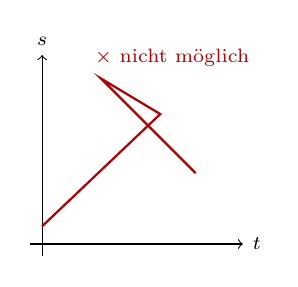
\begin{tikzpicture}[scale=0.75]
  \draw[->] (-0.2,0) -- (3.4,0) node[right] {\scriptsize $t$};
  \draw[->] (0,-0.2) -- (0,3.2) node[above] {\scriptsize $s$};
  \draw[thick,red!70!black] (0,0.3) -- (2,2.2) -- (1,2.8) -- (2.6,1.2);
  \node[red!70!black] at (2.2,3.15) {\scriptsize $\times$ nicht möglich};
\end{tikzpicture}
\\
\footnotesize erlaubt: $t$ nimmt stets zu, $s$ darf auf/ab gehen & \footnotesize nicht erlaubt: Graph läuft zu kleinerem $t$ zurück
\end{tabular}
\end{center}

Das ist ein stärkeres Kriterium als die \textbf{\emph{vertikale}} Linie (bei der $t$
zumindest gleich bleibt, $\Delta t=0$): Hier würde $t$ sogar
\textbf{\emph{abnehmen}} ($\Delta t<0$), was in einem $s$-$t$-Diagramm nie
vorkommen darf.
\end{theoriebox}

\begin{theoriebox}[Lineare Bewegung: Geschwindigkeit als Steigung]
Ist der Graph im $s$-$t$-Diagramm eine \textbf{\emph{Gerade}}, bewegt sich das
Objekt mit \textbf{\emph{konstanter Geschwindigkeit}}: In gleichen Zeitspannen
legt es immer die gleiche Strecke zurück. Eine solche Bewegung mit
konstanter Geschwindigkeit nennt man eine \textbf{\emph{gleichförmige Bewegung}}.
Sie ist im $s$-$t$-Diagramm immer an einer Geraden erkennbar.

Die Geschwindigkeit $v$ ist dann die \textbf{\emph{Steigung}} dieser Geraden:
\[
  v = \frac{\Delta s}{\Delta t} = \frac{s_2 - s_1}{t_2 - t_1}, \qquad
  \text{Einheit von } v \colon\ \si{\meter\per\second}.
\]
Da die Gerade überall gleich steil ist, liefern \textbf{\emph{beliebige}} zwei
Punkte auf ihr denselben Wert für $v$, denn es spielt keine Rolle, welches
Zeitintervall man wählt.

\textbf{Hinweis:} Man schreibt die Formel oft kurz als $v = \dfrac{s}{t}$
(zum Beispiel wenn eine Bewegung bei $s=0$ und $t=0$ beginnt). Gemeint sind
damit aber \textbf{\emph{immer}} eine zurückgelegte Strecke und eine dafür benötigte
Zeit, also \textbf{\emph{Orts- und Zeitdifferenzen}} ($\Delta s$, $\Delta t$),
nie eine einzelne abgelesene Ortskoordinate $s$ oder Uhrzeit $t$. Beginnt
eine Bewegung nicht bei $s=0$ bzw.\ $t=0$, muss deshalb ausdrücklich mit
$\Delta s = s_2-s_1$ und $\Delta t = t_2-t_1$ gerechnet werden, wie im
folgenden Diagramm.

\begin{center}
\begin{tikzpicture}[scale=1.1]
  \draw[->] (-0.3,0) -- (5.7,0) node[right] {\scriptsize $t$ in s};
  \draw[->] (0,-0.3) -- (0,3.7) node[above] {\scriptsize $s$ in m};
  \draw[thick,titleblue] (0,0.4) -- (5,3.4);
  \filldraw[black] (1,1) circle (1.6pt) node[above left] {\scriptsize $(t_1,\,s_1)$};
  \filldraw[black] (4,2.8) circle (1.6pt) node[above left] {\scriptsize $(t_2,\,s_2)$};
  \draw[dashed,accentblue] (1,1) -- (4,1) -- (4,2.8);
  \node[accentblue,below] at (2.5,1) {\scriptsize $\Delta t = t_2-t_1$};
  \node[accentblue,right] at (4,1.9) {\scriptsize $\Delta s = s_2-s_1$};
\end{tikzpicture}
\end{center}

\begin{center}
\begin{tikzpicture}[scale=1.0]
  \draw[->] (-0.3,0) -- (4.7,0) node[right] {\scriptsize $t$};
  \draw[->] (0,-0.3) -- (0,3.7) node[above] {\scriptsize $s$};
  \draw[thick,titleblue] (0,0) -- (4,3.4);
  \draw[thick,accentorange] (0,0) -- (4,1.4);
  \node[titleblue,right] at (4,3.4) {\scriptsize schneller};
  \node[accentorange,right] at (4,1.4) {\scriptsize langsamer};
\end{tikzpicture}
\end{center}

Eine steilere Gerade bedeutet eine grössere Geschwindigkeit.
\end{theoriebox}

\begin{theoriebox}[Einheiten umrechnen: m/s und km/h]
Geschwindigkeiten werden oft auch in $\si{\kilo\meter\per\hour}$ statt in
$\si{\meter\per\second}$ angegeben (z.\,B. beim Autotacho). Für die
Umrechnung braucht man nur zwei Fakten: $\SI{1}{\hour}=\SI{3600}{\second}$
und $\SI{1}{\kilo\meter}=\SI{1000}{\meter}$.

Rechnet man $\SI{1}{\meter\per\second}$ auf eine Stunde hoch, ergibt sich:
\[
  \SI{1}{\meter\per\second}
  = \frac{\SI{3600}{\meter}}{\SI{3600}{\second}}
  = \frac{\SI{3600}{\meter}}{\SI{1}{\hour}}
  = \frac{\SI{3.6}{\kilo\meter}}{\SI{1}{\hour}}
  = \SI{3.6}{\kilo\meter\per\hour}.
\]
Umgekehrt gilt entsprechend $\SI{1}{\kilo\meter\per\hour} = \frac{1}{3.6}\,\si{\meter\per\second}$.

\begin{center}
\begin{tikzpicture}[scale=1.0,>=Latex]
  \node[draw,accentblue,thick,rounded corners,fill=lightblue,minimum width=2.2cm,minimum height=1cm] (ms) at (0,0) {$\si{\meter\per\second}$};
  \node[draw,accentblue,thick,rounded corners,fill=lightblue,minimum width=2.2cm,minimum height=1cm] (kmh) at (5.5,0) {$\si{\kilo\meter\per\hour}$};
  \draw[->,thick,titleblue] (ms.north) to[bend left=35] node[above] {\scriptsize $\times\,3.6$} (kmh.north);
  \draw[->,thick,titleblue] (kmh.south) to[bend left=35] node[below] {\scriptsize $:\,3.6$} (ms.south);
\end{tikzpicture}
\end{center}

Als Formel zusammengefasst:
\[
  v_{\si{\kilo\meter\per\hour}} = v_{\si{\meter\per\second}} \cdot 3.6,
  \qquad
  v_{\si{\meter\per\second}} = v_{\si{\kilo\meter\per\hour}} : 3.6.
\]
\end{theoriebox}

\begin{questions}
\begin{taskbox}[Übung: Steigung ablesen und Einheiten umrechnen]
\question[4] Das folgende $s$-$t$-Diagramm zeigt eine lineare Bewegung. Lies
die Koordinaten der beiden markierten Punkte aus dem Diagramm ab.

\begin{center}
\begin{tikzpicture}[scale=0.55]
  \draw[gray!20] (0,0) grid[xstep=2,ystep=2] (8,10);
  \draw[->] (-0.3,0) -- (8.7,0) node[right] {\scriptsize $t$ in s};
  \draw[->] (0,-0.3) -- (0,10.5) node[above] {\scriptsize $s$ in m};
  \foreach \x in {2,4,6,8} \draw (\x,0.15) -- (\x,-0.15) node[below] {\scriptsize \x};
  \foreach \y/\lbl in {2/4,4/8,6/12,8/16,10/20} \draw (0.15,\y) -- (-0.15,\y) node[left] {\scriptsize \lbl};
  \draw[thick,titleblue] (1,0.5) -- (7,9.5);
  \draw[dashed,gray] (2,0) -- (2,2) -- (0,2);
  \draw[dashed,gray] (6,0) -- (6,8) -- (0,8);
  \filldraw[black] (2,2) circle (1.8pt);
  \filldraw[black] (6,8) circle (1.8pt);
\end{tikzpicture}
\end{center}

\begin{parts}
  \part[2] Berechne die Durchschnittsgeschwindigkeit $v$ als Steigung der
  Geraden. Gib dein Ergebnis in $\si{\meter\per\second}$ an.
  \Antwortraum{2}
  \begin{solution}
  Aus dem Diagramm: $(t_1,s_1)=(\SI{2}{\second},\SI{4}{\meter})$,
  $(t_2,s_2)=(\SI{6}{\second},\SI{16}{\meter})$.
  \[
    v = \frac{\Delta s}{\Delta t} = \frac{\SI{16}{\meter}-\SI{4}{\meter}}{\SI{6}{\second}-\SI{2}{\second}} = \frac{\SI{12}{\meter}}{\SI{4}{\second}} = \SI{3}{\meter\per\second}.
  \]
  \end{solution}
  \part[2] Rechne dein Ergebnis aus Teilaufgabe (a) in
  $\si{\kilo\meter\per\hour}$ um.
  \Antwortraum{2}
  \begin{solution}
  $v = \SI{3}{\meter\per\second} \cdot 3.6 = \SI{10.8}{\kilo\meter\per\hour}$.
  \end{solution}
\end{parts}
\end{taskbox}
\end{questions}

\begin{questions}
\begin{taskbox}[Übung: Blitzer mit Induktionsschleifen]
\question[7] Ein Auto fährt in einer Tempo-30-Zone an einem Blitzer mit
Induktionsschleifen vorbei (Tempolimit: $\SI{30}{\kilo\meter\per\hour}$).
Der Abstand zwischen den beiden Induktionsschleifen beträgt
$\SI{4}{\meter}$.

\begin{center}
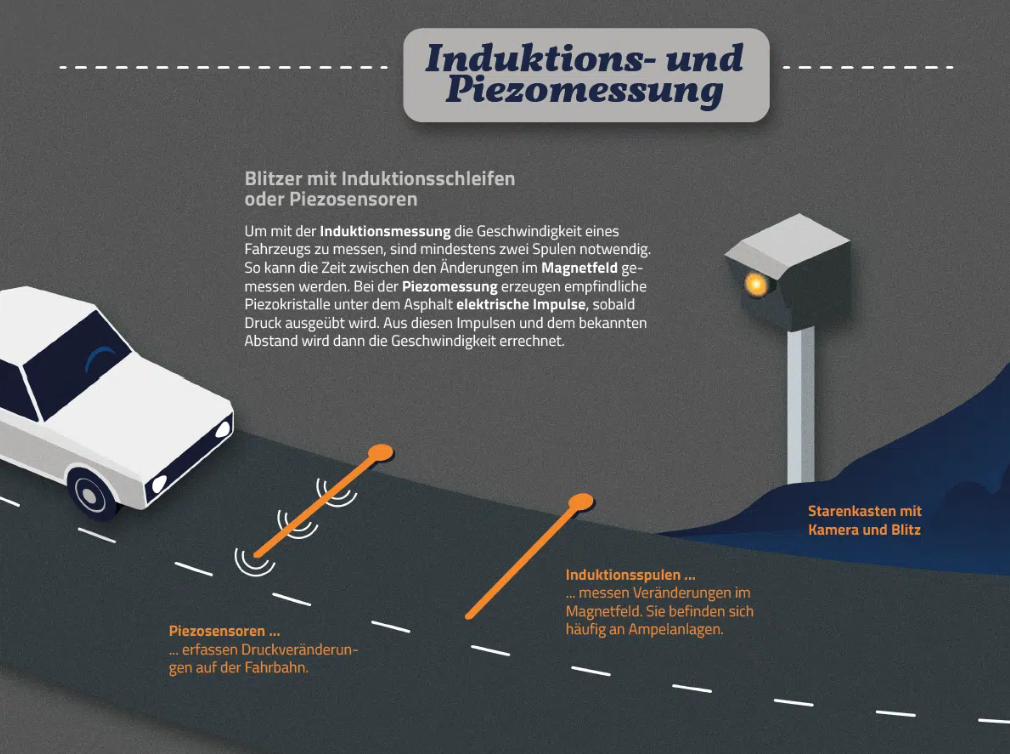
\includegraphics[width=0.7\linewidth]{Bilder/Blitzer_induktionsmessung.png}\\
\footnotesize So misst ein Blitzer mit Induktionsschleifen die Geschwindigkeit.
\end{center}

Die erste Schleife wird bei $t_1=\SI{12.0}{\second}$ ausgelöst (Stoppuhr
seit Messbeginn), die zweite bei $t_2=\SI{12.4}{\second}$.

\begin{parts}
  \part[2] Berechne die Geschwindigkeit des Autos zwischen den beiden
  Schleifen in $\si{\meter\per\second}$ und in
  $\si{\kilo\meter\per\hour}$. Blitzt der Blitzer? Begründe mit einer
  Rechnung.
  \Antwortraum{2}
  \begin{solution}
  $\Delta t = t_2-t_1 = \SI{0.4}{\second}$, $\Delta s = \SI{4}{\meter}$.
  \[
    v = \frac{\Delta s}{\Delta t} = \frac{\SI{4}{\meter}}{\SI{0.4}{\second}} = \SI{10}{\meter\per\second} = \SI{10}{\meter\per\second}\cdot 3.6 = \SI{36}{\kilo\meter\per\hour}.
  \]
  Da $\SI{36}{\kilo\meter\per\hour} > \SI{30}{\kilo\meter\per\hour}$
  (Überschreitung: $\SI{6}{\kilo\meter\per\hour}$), löst der Blitzer aus.
  \end{solution}

  \part[3] Zeichne in das folgende Diagramm sowohl die Bewegung des Autos
  (Teilaufgabe a) als auch die Bewegung, die ein Auto zeigen würde, das
  exakt mit dem Tempolimit fährt, wobei beide Geraden bei der ersten
  Induktionsschleife beginnen. Verwende dazu die relative Zeit
  $t' = t - t_1$, damit beide Geraden bei $t'=\SI{0}{\second}$,
  $s=\SI{0}{\meter}$ starten.

  \begin{center}
  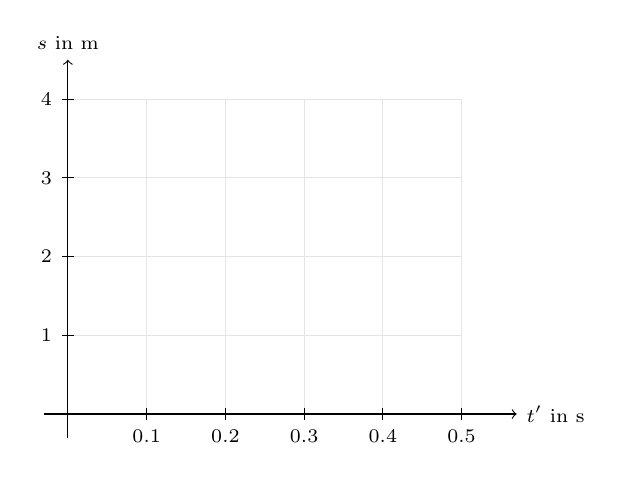
\begin{tikzpicture}[scale=1.0]
    \draw[gray!20] (0,0) grid[xstep=1,ystep=1] (5,4);
    \draw[->] (-0.3,0) -- (5.7,0) node[right] {\scriptsize $t'$ in s};
    \draw[->] (0,-0.3) -- (0,4.5) node[above] {\scriptsize $s$ in m};
    \foreach \x/\lbl in {1/0.1,2/0.2,3/0.3,4/0.4,5/0.5} \draw (\x,0.08) -- (\x,-0.08) node[below] {\scriptsize \lbl};
    \foreach \y in {1,2,3,4} \draw (0.08,\y) -- (-0.08,\y) node[left] {\scriptsize \y};
  \end{tikzpicture}
  \end{center}
  \begin{solution}
  \begin{center}
  \begin{tikzpicture}[scale=1.0]
    \draw[gray!20] (0,0) grid[xstep=1,ystep=1] (5,4);
    \draw[->] (-0.3,0) -- (5.7,0) node[right] {\scriptsize $t'$ in s};
    \draw[->] (0,-0.3) -- (0,4.5) node[above] {\scriptsize $s$ in m};
    \foreach \x/\lbl in {1/0.1,2/0.2,3/0.3,4/0.4,5/0.5} \draw (\x,0.08) -- (\x,-0.08) node[below] {\scriptsize \lbl};
    \foreach \y in {1,2,3,4} \draw (0.08,\y) -- (-0.08,\y) node[left] {\scriptsize \y};
    \draw[thick,accentorange] (0,0) -- (4,4);
    \draw[thick,titleblue] (0,0) -- (4.8,4);
    \filldraw[black] (4,4) circle (1.8pt);
    \filldraw[black] (4.8,4) circle (1.8pt);
  \end{tikzpicture}\\
  \footnotesize \textcolor{accentorange}{Auto}: $\SI{36}{\kilo\meter\per\hour}$ \quad \textcolor{titleblue}{Tempolimit}: $\SI{30}{\kilo\meter\per\hour}$
  \end{center}
  Die Gerade des Autos ist steiler, weil es in derselben Zeit weiter
  kommt als ein Fahrzeug am Tempolimit.
  \end{solution}

  \part[2] Was bedeutet es, wenn eine Bewegung im Diagramm
  \emph{oberhalb} der Geraden des Tempolimits liegt? Und \emph{unterhalb}?
  \Antwortraum{2}
  \begin{solution}
  Oberhalb der Geraden des Tempolimits ist die Steigung grösser als
  deren eigene, also ist die Geschwindigkeit
  $>\SI{30}{\kilo\meter\per\hour}$: das Fahrzeug ist zu schnell
  unterwegs. Unterhalb ist die Steigung kleiner, also die Geschwindigkeit
  $<\SI{30}{\kilo\meter\per\hour}$: das Fahrzeug hält das Tempolimit
  ein.
  \end{solution}
\end{parts}
\end{taskbox}
\end{questions}

\begin{theoriebox}[Der Betrag einer Zahl]
Der \textbf{\emph{Betrag}} $\lvert x\rvert$ einer Zahl $x$ ist ihr \emph{Abstand vom
Nullpunkt} auf der Zahlengeraden. Ganz praktisch: Man streicht einfach
ein vorhandenes Minuszeichen weg. Der Betrag ist deshalb nie negativ.

\begin{center}
\begin{tikzpicture}[scale=0.9]
  \draw[->] (-3.3,0) -- (3.3,0);
  \foreach \x in {-3,-2,-1,0,1,2,3} \draw (\x,0.08) -- (\x,-0.08) node[below] {\scriptsize \x};
  \filldraw[titleblue] (-2,0) circle (1.8pt);
  \filldraw[accentorange] (2,0) circle (1.8pt);
  \draw[<->,titleblue] (-2,0.5) -- (0,0.5) node[midway,above] {\scriptsize $2$};
  \draw[<->,accentorange] (0,-0.5) -- (2,-0.5) node[midway,below] {\scriptsize $2$};
\end{tikzpicture}
\end{center}

$-2$ und $2$ liegen beide genau $2$ Schritte vom Nullpunkt entfernt,
nur in entgegengesetzte Richtungen. Deshalb gilt $\lvert -2\rvert =
\lvert 2\rvert = 2$: gleicher Betrag, unterschiedliches Vorzeichen.

Bei einer Geschwindigkeit $v$ gibt der Betrag $\lvert v\rvert$ deshalb an,
\textbf{\emph{wie schnell}} sich ein Objekt bewegt, unabhängig davon, ob es
vorwärts oder rückwärts unterwegs ist.
\end{theoriebox}

\begin{theoriebox}[Die drei Grundbewegungen]
Bei linearer Bewegung gibt das \textbf{\emph{Vorzeichen}} der Steigung die
Richtung an:

\begin{center}
\begin{tabular}{@{}ccc@{}}
\begin{tikzpicture}[scale=0.75]
  \draw[->] (-0.2,0) -- (2.8,0) node[right] {\scriptsize $t$};
  \draw[->] (0,-0.2) -- (0,2.8) node[above] {\scriptsize $s$};
  \draw[thick,accentblue] (0,1.4) -- (2.5,1.4);
\end{tikzpicture}
&
\begin{tikzpicture}[scale=0.75]
  \draw[->] (-0.2,0) -- (2.8,0) node[right] {\scriptsize $t$};
  \draw[->] (0,-0.2) -- (0,2.8) node[above] {\scriptsize $s$};
  \draw[thick,accentblue] (0,0.2) -- (2.5,2.5);
\end{tikzpicture}
&
\begin{tikzpicture}[scale=0.75]
  \draw[->] (-0.2,0) -- (2.8,0) node[right] {\scriptsize $t$};
  \draw[->] (0,-0.2) -- (0,2.8) node[above] {\scriptsize $s$};
  \draw[thick,accentblue] (0,2.5) -- (2.5,0.2);
\end{tikzpicture}
\\
\footnotesize \textbf{Anhalten} & \footnotesize \textbf{Vorwärtsbewegung} & \footnotesize \textbf{Rückwärtsbewegung}
\\
\footnotesize Steigung $=0$ & \footnotesize Steigung $>0$ & \footnotesize Steigung $<0$
\\
\footnotesize $v=0$ & \footnotesize $v>0$ & \footnotesize $v<0$
\end{tabular}
\end{center}

Beim \textbf{\emph{Anhalten}} (auch: \textbf{\emph{Ruhe}}) bleibt der Ort konstant, die
Gerade ist waagrecht. Bei der \textbf{\emph{Vorwärtsbewegung}} nimmt $s$ mit der
Zeit zu, bei der \textbf{\emph{Rückwärtsbewegung}} nimmt $s$ ab: Der Betrag
$\lvert v\rvert$ sagt, \textbf{\emph{wie schnell}}, das Vorzeichen sagt, \emph{in
welche Richtung}.
\end{theoriebox}

\needspace{45\baselineskip}
\begin{questions}
\begin{taskbox}[Kurzaufgabe: Vertikale Linie]
\question[3] Ein Schüler zeichnet das folgende $s$-$t$-Diagramm:

\begin{center}
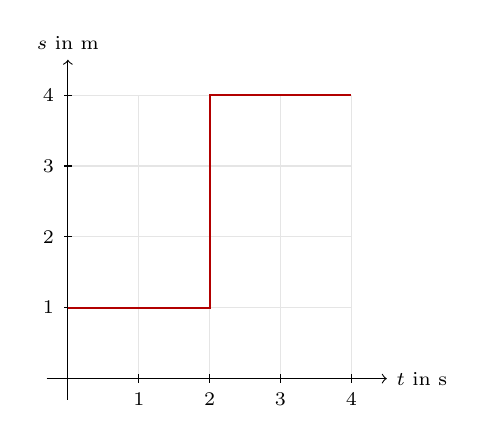
\begin{tikzpicture}[scale=0.9]
  \draw[gray!20] (0,0) grid (4,4);
  \draw[->] (-0.3,0) -- (4.5,0) node[right] {\scriptsize $t$ in s};
  \draw[->] (0,-0.3) -- (0,4.5) node[above] {\scriptsize $s$ in m};
  \foreach \x in {1,2,3,4} \draw (\x,0.06) -- (\x,-0.06) node[below] {\scriptsize \x};
  \foreach \y in {1,2,3,4} \draw (0.06,\y) -- (-0.06,\y) node[left] {\scriptsize \y};
  \draw[thick,red!70!black] (0,1) -- (2,1) -- (2,4) -- (4,4);
\end{tikzpicture}
\end{center}

Erkläre, weshalb der senkrechte Abschnitt bei $t=\SI{2}{\second}$
physikalisch keinen Sinn macht.
\Antwortraum{3}

\begin{solution}
Der senkrechte Abschnitt würde bedeuten, dass sich das Objekt in null Zeit
($\Delta t=0$) von $s=\SI{1}{\meter}$ nach $s=\SI{4}{\meter}$ bewegt
($\Delta s=\SI{3}{\meter}\neq 0$). Die Geschwindigkeit $v=\Delta s/\Delta t$
wäre dann unendlich gross. Das ist physikalisch nicht möglich.
\end{solution}
\end{taskbox}
\end{questions}

\begin{theoriebox}[Bewegungsabschnitte im kombinierten Diagramm]
Die meisten Bewegungen bestehen nicht nur aus einem einzigen der obigen
Fälle, sondern setzen sich aus mehreren linearen Abschnitten zusammen.
Zwischen zwei Knicken (Richtungs- oder Geschwindigkeitswechseln) bleibt
die Steigung konstant. Man liest jeden Abschnitt einzeln wie eine
eigene Gerade und ordnet ihm eine der drei Grundbewegungen zu.

\begin{center}
\begin{tikzpicture}[scale=0.9]
  \draw[gray!20] (0,0) grid[xstep=2,ystep=1] (8,4);
  \draw[->] (-0.3,0) -- (9.7,0) node[right] {$t$ in s};
  \draw[->] (0,-0.3) -- (0,5.5) node[above] {$s$ in m};
  \foreach \x in {2,4,6,8} \draw (\x,0.08) -- (\x,-0.08) node[below] {\scriptsize \x};
  \foreach \y in {1,2,3,4} \draw (0.08,\y) -- (-0.08,\y) node[left] {\scriptsize \y};
  \draw[thick,titleblue] (0,0.5) -- (3,3.5) -- (5,3.5) -- (9,1.5);
  \draw[dashed,gray] (3,0) -- (3,3.5);
  \draw[dashed,gray] (5,0) -- (5,3.5);
  \node[accentblue,above left] at (1.5,2) {\footnotesize vorwärts};
  \node[accentblue,above] at (4,3.6) {\footnotesize Stillstand};
  \node[accentblue,below] at (7,2.2) {\footnotesize rückwärts};
\end{tikzpicture}
\end{center}

An jedem Knick ändert sich die Steigung (also die Geschwindigkeit)
sprunghaft; zwischen zwei Knicken bleibt sie konstant.
\end{theoriebox}

\begin{beispielbox}[Beispiel: Raststätte auf der Autobahn]
Ein Auto fährt auf der Autobahn mit $\SI{120}{\kilo\meter\per\hour}$. Nach
$t=\SI{15}{\minute}$ (zurückgelegte Strecke: $\SI{30}{\kilo\meter}$) fährt
es bei einer Raststätte ab, um eine Pause einzulegen und etwas zu essen.
Die Pause dauert $\SI{9}{\minute}$; währenddessen bleibt der Ort $s$
konstant. Danach fährt das Auto wieder auf die Autobahn, wo zunächst
weiterhin $\SI{120}{\kilo\meter\per\hour}$ erlaubt sind. Nach
$\SI{6}{\minute}$ verlässt es die Autobahn über eine Ausfahrt und fährt
dort für $\SI{6}{\minute}$ mit $\SI{60}{\kilo\meter\per\hour}$ weiter,
allerdings in die falsche Richtung! An der nächsten Kreuzung wendet es und
fährt auf einer Hauptstrasse mit $\SI{80}{\kilo\meter\per\hour}$ die
restlichen $\SI{9}{\minute}$ in die \emph{entgegengesetzte} Richtung zurück
in Richtung Ausgangspunkt ($s=\SI{0}{\kilo\meter}$ ist dabei nur der
willkürlich gewählte Nullpunkt der Autobahnkilometrierung, nicht
\emph{zuhause}).

\begin{center}
\begin{tikzpicture}[scale=0.78]
  \draw[gray!20] (0,0) grid[xstep=1,ystep=1] (15,5);
  \draw[->] (-0.3,0) -- (15.7,0) node[right] {\scriptsize $t$ in min};
  \draw[->] (0,-0.3) -- (0,5.5) node[above] {\scriptsize $s$ in km};
  \foreach \x/\lbl in {0/0,5/15,8/24,10/30,12/36,15/45} \draw (\x,0.08) -- (\x,-0.08) node[below] {\scriptsize \lbl};
  \foreach \y/\lbl in {0/0,1/10,2/20,3/30,4/40,5/50} \draw (0.08,\y) -- (-0.08,\y) node[left] {\scriptsize \lbl};
  \draw[thick,titleblue] (0,0) -- (5,3) -- (8,3) -- (10,4.2) -- (12,4.8) -- (15,3.6);
  \draw[dashed,gray] (5,0) -- (5,3);
  \draw[dashed,gray] (8,0) -- (8,3);
  \draw[dashed,gray] (10,0) -- (10,4.2);
  \draw[dashed,gray] (12,0) -- (12,4.8);
  \filldraw[accentblue] (0,0) circle (1.6pt);
  \filldraw[accentblue] (5,3) circle (1.6pt);
  \filldraw[accentblue] (8,3) circle (1.6pt);
  \filldraw[accentblue] (10,4.2) circle (1.6pt);
  \filldraw[accentblue] (12,4.8) circle (1.6pt);
  \filldraw[accentblue] (15,3.6) circle (1.6pt);
  \node[accentblue,above left] at (2.5,1.5) {\footnotesize \SI{120}{\kilo\meter\per\hour}};
  \node[accentblue,above] at (6.5,3) {\footnotesize Pause};
  \node[accentblue,above left] at (9,3.6) {\footnotesize \SI{120}{\kilo\meter\per\hour}};
  \node[accentblue,above] at (11,4.5) {\footnotesize \SI{60}{\kilo\meter\per\hour}};
  \node[accentblue,above right] at (13.5,4.2) {\footnotesize $-\SI{80}{\kilo\meter\per\hour}$};
\end{tikzpicture}

\footnotesize $t=\SI{0}{\minute}$: $s=\SI{0}{\kilo\meter}$ \quad
$t=\SI{15}{\minute}$: $s=\SI{30}{\kilo\meter}$ (Ankunft Raststätte) \quad
$t=\SI{24}{\minute}$: $s=\SI{30}{\kilo\meter}$ (Weiterfahrt)\\
$t=\SI{30}{\minute}$: $s=\SI{42}{\kilo\meter}$ (Ausfahrt) \quad
$t=\SI{36}{\minute}$: $s=\SI{48}{\kilo\meter}$ (Wende) \quad
$t=\SI{45}{\minute}$: $s=\SI{36}{\kilo\meter}$ (Ende der Fahrt)
\end{center}

Vergleiche die beiden $\SI{120}{\kilo\meter\per\hour}$-Abschnitte: Obwohl
sie an unterschiedlichen Stellen im Diagramm liegen, ist ihre Steigung
gleich gross: Gleiche Geschwindigkeit bedeutet immer gleiche Steigung.
Der $\SI{60}{\kilo\meter\per\hour}$-Abschnitt ist dagegen \emph{weniger
steil} (halb so schnell wie auf der Autobahn, also auch nur halb so grosse
Steigung). Der letzte Abschnitt hat sogar eine \emph{negative} Steigung:
Das Vorzeichen zeigt, dass sich das Auto jetzt in die entgegengesetzte
Richtung bewegt: Der Ort $s$ nimmt ab, obwohl der Betrag der
Geschwindigkeit ($\SI{80}{\kilo\meter\per\hour}$) sogar grösser ist als
beim vorherigen Abschnitt.
\end{beispielbox}

\begin{beispielbox}[Beispiel: Zwei Personen begegnen sich]
Zwei Personen gehen von entgegengesetzten Enden eines $\SI{20}{\meter}$
langen, geraden Wegs aufeinander zu. Person A startet bei
$s=\SI{0}{\meter}$ und geht mit $v_A=\SI{1}{\meter\per\second}$ in
positiver Richtung; Person B startet bei $s=\SI{20}{\meter}$ und geht mit
$v_B=\SI{-1.5}{\meter\per\second}$ (also in negativer Richtung, auf Person
A zu). Da keine der beiden anhält, begegnen sich beide unterwegs und gehen
anschliessend unverändert weiter. Im Diagramm zeigt sich das als zwei
Geraden, die sich in genau einem Punkt kreuzen.

\begin{center}
\begin{tikzpicture}[scale=0.85]
  \draw[gray!20] (0,0) grid (10,5);
  \draw[->] (-0.3,0) -- (10.7,0) node[right] {\scriptsize $t$ in s};
  \draw[->] (0,-0.3) -- (0,5.7) node[above] {\scriptsize $s$ in m};
  \foreach \x in {2,4,6,8,10} \draw (\x,0.06) -- (\x,-0.06) node[below] {\scriptsize \x};
  \foreach \y/\lbl in {1/4,2/8,3/12,4/16,5/20} \draw (0.06,\y) -- (-0.06,\y) node[left] {\scriptsize \lbl};
  \draw[thick,accentorange] (0,0) -- (10,2.5) node[right] {\scriptsize Person A};
  \draw[thick,titleblue] (0,5) -- (10,1.25) node[right] {\scriptsize Person B};
  \filldraw[black] (8,2) circle (1.8pt);
\end{tikzpicture}

\footnotesize Treffpunkt: $t=\SI{8}{\second}$, $s=\SI{8}{\meter}$
\end{center}
\end{beispielbox}

\begin{questions}
\begin{taskbox}[Übung: Bildfahrplan mit drei Zügen]
\question[9] Auf der Strecke zwischen Zürich HB und Luzern verkehren gleichzeitig
drei Züge. Der folgende Bildfahrplan zeigt ihre Bewegung:

\begin{center}
\begin{tikzpicture}[scale=0.85]
  \draw[gray!15] (0,0) grid[xstep=1,ystep=1] (12,11);
  \draw[gray!45] (0,2.4) -- (12,2.4);
  \draw[gray!45] (0,7) -- (12,7);
  \draw[->] (-0.3,0) -- (12.7,0) node[right] {\scriptsize $t$ in min};
  \draw[->] (0,-0.3) -- (0,11.7) node[above] {\scriptsize $s$};
  \foreach \x/\lbl in {0/0,2/10,4/20,6/30,8/40,10/50,12/60} \draw (\x,0.1) -- (\x,-0.1) node[below] {\scriptsize \lbl};
  \foreach \y/\lbl in {0/Zürich HB,2.4/Thalwil,7/Zug,11/Luzern} \draw (0.1,\y) -- (-0.1,\y) node[left] {\scriptsize \lbl};
  \draw[thick,titleblue] (0,0) -- (8,11) node[above left] {\scriptsize Zug 1 (IR)};
  \draw[thick,accentorange] (1,0) -- (3,2.4) -- (3.4,2.4) -- (7,7) -- (7.6,7) -- (11.6,11) node[left] {\scriptsize Zug 2 (S-Bahn)};
  \draw[thick,accentpurple] (2,11) node[right] {\scriptsize Zug 3 (IC)} -- (11,0);
\end{tikzpicture}
\end{center}

\begin{parts}
  \part[1] Lies aus dem Diagramm ab: Nach wie vielen Minuten kommt Zug 1
  (IR) in Luzern an?
  \Antwortraum{1}
  \begin{solution}
  Nach $t=\SI{40}{\minute}$.
  \end{solution}

  \part[2] Berechne die Geschwindigkeit von Zug 1 (IR) zwischen Zürich HB
  und Luzern in $\si{\kilo\meter\per\hour}$. Die Strecke ist
  $\SI{55}{\kilo\meter}$ lang.
  \Antwortraum{2}
  \begin{solution}
  \[
    v = \frac{\SI{55}{\kilo\meter}}{\SI{40}{\minute}} = \SI{1.375}{\kilo\meter\per\minute} = \SI{1.375}{\kilo\meter\per\minute}\cdot 60 = \SI{82.5}{\kilo\meter\per\hour}.
  \]
  \end{solution}

  \part[2] Zug 2 (S-Bahn) hält unterwegs zweimal. Lies aus dem Diagramm
  ab: An welchen Stationen, und wie lange dauert jeder Halt?
  \Antwortraum{2}
  \begin{solution}
  Halt in Thalwil: $t=\SI{15}{\minute}$ bis $t=\SI{17}{\minute}$, also
  $\SI{2}{\minute}$. Halt in Zug: $t=\SI{35}{\minute}$ bis
  $t=\SI{38}{\minute}$, also $\SI{3}{\minute}$.
  \end{solution}

  \part[2] Zug 1 (IR) und Zug 3 (IC) begegnen sich unterwegs. Bestimme
  Zeitpunkt und Ort dieser Begegnung möglichst genau aus dem Diagramm.
  \Antwortraum{2}
  \begin{solution}
  Die Geraden kreuzen sich bei etwa $t\approx\SI{26}{\minute}$,
  $s\approx\SI{36}{\kilo\meter}$ (bei der Station Zug).
  \end{solution}

  \part[2] Woran erkennt man im Diagramm, dass Zug 3 (IC) in die
  \emph{Gegenrichtung} fährt (Luzern$\to$Zürich HB statt Zürich
  HB$\to$Luzern)? Welcher der drei Züge ist unterwegs am schnellsten?
  \Antwortraum{2}
  \begin{solution}
  Die Gerade von Zug 3 hat eine \emph{negative} Steigung ($s$ nimmt mit
  der Zeit ab): Das Vorzeichen zeigt die entgegengesetzte Richtung an.
  Am schnellsten ist Zug 1 (IR): Seine Gerade ist am steilsten (grösster
  Betrag der Steigung, $\SI{82.5}{\kilo\meter\per\hour}$).
  \end{solution}
\end{parts}
\end{taskbox}
\end{questions}

\begin{questions}
\begin{groupbox}[Partnerarbeit: Bewegungsgeschichte zeichnen]
\question[6] Bildet Zweiergruppen. Überlegt euch \emph{einzeln} (ohne
miteinander zu sprechen) eine eigene Bewegungsgeschichte zu einem selbst
gewählten Objekt (zum Beispiel ein Zug, ein Tier, ein Flugzeug, ein
Fahrstuhl, ein Skifahrer, \ldots). Die Bewegung soll möglichst
\emph{abwechslungsreich} sein: mindestens drei verschiedene Abschnitte
(z.\,B. Vorwärtsbewegung, Stillstand, Rückwärtsbewegung, unterschiedlich
schnelle Abschnitte, \ldots). Wählt für $t$ und $s$ Einheiten, die zu
eurem Szenario passen (z.\,B. \si{\kilo\meter} und \si{\hour} für einen
Zug, \si{\meter} und \si{\second} für ein Tier).

\begin{parts}
  \part[3] Zeichne dein eigenes $s$-$t$-Diagramm in \emph{Diagramm 1}
  (deine Partnerin/dein Partner darf es noch nicht sehen). Beschrifte die
  Achsen mit den Einheiten, die du gewählt hast.

  % Verhindert, dass "Diagramm 1" oben auf der Seite als Titelzeile
  % verwaist, während das zugehörige Diagramm erst auf der Folgeseite
  % erscheint (analog zum \needspace vor der taskbox "Kurzaufgabe:
  % Vertikale Linie" weiter oben im Dokument).
  \needspace{8.5cm}
  \begin{center}
  \textbf{Diagramm 1 (eigene Bewegungsgeschichte)}\\[0.3em]
  \begin{tikzpicture}[scale=1.08]
    \draw[gray!20] (0,0) grid (10,6);
    \draw[->] (-0.3,0) -- (10.5,0) node[right] {\scriptsize $t$ in \underline{\hspace{1.1cm}}};
    \draw[->] (0,-0.3) -- (0,6.5) node[above] {\scriptsize $s$ in \underline{\hspace{1.1cm}}};
  \end{tikzpicture}
  \end{center}

  \part[3] Beschreibe deiner Partnerin/deinem Partner die
  Bewegungsgeschichte \emph{nur mit Worten} (ohne das Diagramm zu
  zeigen). Sie/er zeichnet daraufhin, was verstanden wurde, in
  \emph{Diagramm 2}. Vergleicht anschliessend beide Diagramme: Stimmen
  sie überein? Wo gab es Missverständnisse, und woran lag das?

  \begin{center}
  \textbf{Diagramm 2 (von der Partnerin/vom Partner gezeichnet)}\\[0.3em]
  \begin{tikzpicture}[scale=1.08]
    \draw[gray!20] (0,0) grid (10,6);
    \draw[->] (-0.3,0) -- (10.5,0) node[right] {\scriptsize $t$ in \underline{\hspace{1.1cm}}};
    \draw[->] (0,-0.3) -- (0,6.5) node[above] {\scriptsize $s$ in \underline{\hspace{1.1cm}}};
  \end{tikzpicture}
  \end{center}
\end{parts}
\end{groupbox}
\end{questions}

\begin{theoriebox}[Durchschnitts- und Momentangeschwindigkeit]
Bisher haben wir bei einer Bewegung immer die Sekantensteigung zwischen
zwei Punkten berechnet:
\[
  \bar v = \frac{\Delta s}{\Delta t} = \frac{s_2-s_1}{t_2-t_1}.
\]
Das ist die \textbf{\emph{Durchschnittsgeschwindigkeit}}. Sie sagt nur etwas über
den gesamten Zeitraum von $t_1$ bis $t_2$ aus, nicht darüber, wie schnell
sich das Objekt zu einem einzelnen Zeitpunkt \textbf{\emph{dazwischen}} tatsächlich
bewegt hat.

Manchmal will man aber wissen, wie schnell sich ein Objekt genau
\textbf{\emph{jetzt}}, zu einem bestimmten Zeitpunkt $t_0$, bewegt. Das nennt man
die \textbf{\emph{Momentangeschwindigkeit}} $v(t_0)$.

\begin{itemize}[leftmargin=1.2cm,itemsep=0.4em]
  \item Ist der Graph im $s$-$t$-Diagramm eine \textbf{\emph{Gerade}} (wie in
  diesem Arbeitsblatt bisher immer), ist die Steigung überall gleich:
  Momentan- und Durchschnittsgeschwindigkeit sind dann identisch, egal
  welches Zeitintervall man wählt.
  \item Ist der Graph dagegen \textbf{\emph{gekrümmt}} (Bewegung mit sich
  ändernder Geschwindigkeit, z.\,B. bei einer Beschleunigung), ändert
  sich die Steigung von Punkt zu Punkt. Um die Momentangeschwindigkeit an
  einem einzelnen Punkt zu bestimmen, zeichnet man dort die
  \textbf{\emph{Tangente}} (die Gerade, die den Graphen genau an diesem Punkt
  berührt, ohne ihn zu schneiden) und liest deren Steigung ab.
\end{itemize}

\begin{center}
\begin{tikzpicture}[scale=0.9]
  \draw[->] (-0.3,0) -- (6.7,0) node[right] {\scriptsize $t$};
  \draw[->] (0,-0.3) -- (0,6) node[above] {\scriptsize $s$};
  \draw[thick,titleblue,domain=0:6,samples=60,smooth] plot (\x,{0.15*\x*\x});
  \draw[thick,accentorange] (1,0.15) -- (5,3.75) node[right] {\scriptsize Sekante: $\bar v$};
  \draw[thick,accentpurple] (2.5,0.6) -- (5.5,4.2) node[right] {\scriptsize Tangente: $v(t_0)$};
  \filldraw[black] (1,0.15) circle (1.6pt);
  \filldraw[black] (5,3.75) circle (1.6pt);
  \filldraw[black] (4,2.4) circle (1.6pt);
  \draw (1,0.05) -- (1,-0.05) node[below] {\scriptsize $t_1$};
  \draw (4,0.05) -- (4,-0.05) node[below] {\scriptsize $t_0$};
  \draw (5,0.05) -- (5,-0.05) node[below] {\scriptsize $t_2$};
\end{tikzpicture}
\end{center}

Je näher $t_1$ und $t_2$ zusammenrücken ($\Delta t \to 0$), desto mehr
nähert sich die Sekante der Tangente an einem der beiden Punkte an.
Deshalb gilt: Die Momentangeschwindigkeit ist der Grenzwert der
Durchschnittsgeschwindigkeit für $\Delta t \to 0$.

\textbf{Wichtig für die folgende Aufgabe:} Wir bleiben in diesem
Arbeitsblatt bei \textbf{\emph{stückweise linearen}} (geraden) $s$-$t$-Diagrammen.
Auf einem einzelnen Geradenstück lässt sich die Momentangeschwindigkeit an
jedem Punkt direkt und exakt als Steigung \textbf{\emph{dieses}} Geradenstücks
ablesen, ganz ohne Tangente zeichnen zu müssen. Betrachtet man aber ein
Zeitintervall, das über einen \textbf{\emph{Knick}} (Richtungs- oder
Geschwindigkeitswechsel) hinausgeht, unterscheiden sich Momentan- und
Durchschnittsgeschwindigkeit trotzdem, wie das folgende Beispiel zeigt.
\end{theoriebox}

\begin{questions}
\begin{taskbox}[Übung: Momentan- vs. Durchschnittsgeschwindigkeit]
\question[9] Ein Aufzug in einem Bürogebäude bewegt sich wie im folgenden
Diagramm gezeigt ($s$ = Höhe über dem Erdgeschoss).

\begin{center}
\begin{tikzpicture}[scale=0.3]
  \draw[gray!20] (0,0) grid[xstep=4,ystep=3] (32,18);
  \draw[->] (-1,0) -- (33,0) node[right] {\scriptsize $t$ in s};
  \draw[->] (0,-1) -- (0,19) node[above] {\scriptsize $s$ in m};
  \foreach \x in {0,8,14,20,26,32} \draw (\x,0.3) -- (\x,-0.3) node[below] {\scriptsize \x};
  \foreach \y in {0,3,6,9,12,15,18} \draw (0.3,\y) -- (-0.3,\y) node[left] {\scriptsize \y};
  \draw[thick,titleblue] (0,0) -- (8,12) -- (14,12) -- (20,18) -- (32,3);
  \filldraw[black] (0,0) circle (1.6pt);
  \filldraw[black] (8,12) circle (1.6pt);
  \filldraw[black] (14,12) circle (1.6pt);
  \filldraw[black] (20,18) circle (1.6pt);
  \filldraw[black] (32,3) circle (1.6pt);
  \filldraw[accentorange] (4,6) circle (2pt) node[above left] {\scriptsize $A$};
  \filldraw[accentorange] (10,12) circle (2pt) node[above] {\scriptsize $B$};
  \filldraw[accentorange] (17,15) circle (2pt) node[above] {\scriptsize $C$};
  \filldraw[accentorange] (26,10.5) circle (2pt) node[above right] {\scriptsize $D$};
\end{tikzpicture}
\end{center}

\begin{parts}
  \part[4] Bestimme die Momentangeschwindigkeit des Aufzugs zu den vier
  markierten Zeitpunkten $A$ ($t=\SI{4}{\second}$), $B$
  ($t=\SI{10}{\second}$), $C$ ($t=\SI{17}{\second}$) und $D$
  ($t=\SI{26}{\second}$).
  \Antwortraum{4}
  \begin{solution}
  Alle vier Punkte liegen jeweils auf einem einzelnen Geradenstück. Dort
  ist die Momentangeschwindigkeit exakt gleich der Steigung dieses
  Geradenstücks:
  \begin{itemize}
    \item[$A$:] $v = \dfrac{\SI{12}{\meter}-\SI{0}{\meter}}{\SI{8}{\second}-\SI{0}{\second}} = \SI{1.5}{\meter\per\second}$
    \item[$B$:] $v = \SI{0}{\meter\per\second}$ (Aufzug steht still, Türen offen)
    \item[$C$:] $v = \dfrac{\SI{18}{\meter}-\SI{12}{\meter}}{\SI{20}{\second}-\SI{14}{\second}} = \SI{1}{\meter\per\second}$
    \item[$D$:] $v = \dfrac{\SI{3}{\meter}-\SI{18}{\meter}}{\SI{32}{\second}-\SI{20}{\second}} = -\SI{1.25}{\meter\per\second}$
  \end{itemize}
  \end{solution}

  \part[2] Bestimme die Durchschnittsgeschwindigkeit (a) zwischen $t=0$
  und $t=\SI{8}{\second}$ und (b) zwischen $t=0$ und $t=\SI{32}{\second}$
  (der ganzen Fahrt).
  \Antwortraum{2}
  \begin{solution}
  (a) $\bar v = \dfrac{\SI{12}{\meter}-\SI{0}{\meter}}{\SI{8}{\second}} = \SI{1.5}{\meter\per\second}$,
  identisch mit der Momentangeschwindigkeit bei $A$, weil dieses
  Intervall vollständig auf einem einzigen Geradenstück liegt.\\
  (b) $\bar v = \dfrac{\SI{3}{\meter}-\SI{0}{\meter}}{\SI{32}{\second}} \approx \SI{0.09}{\meter\per\second}$.
  \end{solution}

  \part[1] Vergleiche das Ergebnis aus Teilaufgabe (b) mit den vier
  Momentangeschwindigkeiten aus Teilaufgabe (a): Bewegt sich der Aufzug
  über die ganze Fahrt gesehen mit derselben Geschwindigkeit wie zu
  irgendeinem der vier Zeitpunkte $A$ bis $D$?
  \Antwortraum{1}
  \begin{solution}
  Nein. $\bar v \approx \SI{0.09}{\meter\per\second}$ ist viel kleiner als
  alle vier Momentangeschwindigkeiten. Der Aufzug bewegt sich zu
  \emph{keinem} Zeitpunkt der Fahrt tatsächlich mit dieser Geschwindigkeit.
  Die Durchschnittsgeschwindigkeit über die ganze Fahrt ist also keine
  \glqq typische\grqq{} Momentangeschwindigkeit, sondern hängt nur von
  Start- und Endpunkt ab.
  \end{solution}

  \part[2] Zeichne im Diagramm die Gerade ein, die den Start- und den
  Endpunkt der Fahrt ($t=0$ und $t=\SI{32}{\second}$) direkt verbindet.
  Erkläre, was diese Gerade darstellt.
  \Antwortraum{2}
  \begin{solution}
  \begin{center}
  \begin{tikzpicture}[scale=0.3]
    \draw[gray!20] (0,0) grid[xstep=4,ystep=3] (32,18);
    \draw[->] (-1,0) -- (33,0) node[right] {\scriptsize $t$ in s};
    \draw[->] (0,-1) -- (0,19) node[above] {\scriptsize $s$ in m};
    \foreach \x in {0,8,14,20,26,32} \draw (\x,0.3) -- (\x,-0.3) node[below] {\scriptsize \x};
    \foreach \y in {0,3,6,9,12,15,18} \draw (0.3,\y) -- (-0.3,\y) node[left] {\scriptsize \y};
    \draw[thick,titleblue] (0,0) -- (8,12) -- (14,12) -- (20,18) -- (32,3);
    \draw[thick,accentpurple,dashed] (0,0) -- (32,3) node[right] {\scriptsize Sekante: $\bar v$};
    \filldraw[black] (0,0) circle (1.6pt);
    \filldraw[black] (8,12) circle (1.6pt);
    \filldraw[black] (14,12) circle (1.6pt);
    \filldraw[black] (20,18) circle (1.6pt);
    \filldraw[black] (32,3) circle (1.6pt);
  \end{tikzpicture}
  \end{center}
  Diese Gerade beschreibt eine \emph{gedachte} gleichförmige Bewegung mit
  konstanter Geschwindigkeit $\bar v\approx\SI{0.09}{\meter\per\second}$,
  die in derselben Zeit ($\SI{32}{\second}$) genau dieselbe Ortsänderung
  ($\SI{3}{\meter}$) zurücklegen würde wie der tatsächliche (viel
  kompliziertere) Aufzugsweg. Die Steigung der Sekante beschreibt also den
  \emph{direkten Weg} zwischen Start- und Endpunkt einer Bewegung im
  selben Zeitintervall, unabhängig davon, was dazwischen tatsächlich
  passiert ist.
  \end{solution}
\end{parts}
\end{taskbox}
\end{questions}

\begin{questions}
\begin{taskbox}[Übung: Momentan- und Durchschnittsgeschwindigkeit an einer Kurve]
\question[8] Eine Kugel rollt eine schiefe Ebene (Rampe) hinunter und wird
dabei kontinuierlich schneller. Ihre Position wurde regelmässig gemessen;
das ergibt das folgende (gekrümmte) $s$-$t$-Diagramm. Bei $P$
($t=\SI{2}{\second}$) befindet sich die Kugel bei $s=\SI{2}{\meter}$, bei
$Q$ ($t=\SI{5}{\second}$) bei $s=\SI{12.5}{\meter}$.

\begin{center}
\begin{tikzpicture}[scale=0.95]
  \draw[gray!20] (0,0) grid[xstep=1,ystep=1] (6,6);
  \draw[->] (-0.3,0) -- (6.7,0) node[right] {\scriptsize $t$ in s};
  \draw[->] (0,-0.3) -- (0,6.7) node[above] {\scriptsize $s$ in m};
  \foreach \x in {0,1,2,3,4,5,6} \draw (\x,0.1) -- (\x,-0.1) node[below] {\scriptsize \x};
  \foreach \y/\lbl in {0/0,1/3,2/6,3/9,4/12,5/15,6/18} \draw (0.1,\y) -- (-0.1,\y) node[left] {\scriptsize \lbl};
  \draw[thick,titleblue,domain=0:6,samples=60,smooth] plot (\x,{(\x*\x)/6});
  \filldraw[accentorange] (2,0.667) circle (2pt) node[below right] {\scriptsize $P$};
  \filldraw[accentorange] (5,4.167) circle (2pt) node[above left] {\scriptsize $Q$};
\end{tikzpicture}
\end{center}

\begin{parts}
  \part[2] Bestimme die Durchschnittsgeschwindigkeit zwischen $P$ und
  $Q$.
  \Antwortraum{2}
  \begin{solution}
  $\bar v = \dfrac{\SI{12.5}{\meter}-\SI{2}{\meter}}{\SI{5}{\second}-\SI{2}{\second}} = \dfrac{\SI{10.5}{\meter}}{\SI{3}{\second}} = \SI{3.5}{\meter\per\second}$.
  \end{solution}

  \part[2] Zeichne bei $P$ mit einem Lineal möglichst genau die Tangente
  an die Kurve ein. Lies an deiner Tangente zwei gut ablesbare Punkte ab
  und bestimme daraus die Momentangeschwindigkeit bei $P$.
  \Antwortraum{2}
  \begin{solution}
  Deine Zeichnung wird nicht exakt mit der folgenden Lösung
  übereinstimmen. Das ist normal, die Tangente wird nur qualitativ
  abgeschätzt. Werte zwischen etwa $\SI{1.5}{\meter\per\second}$ und
  $\SI{2.5}{\meter\per\second}$ gelten als korrekt abgelesen; die exakte
  Tangente ergibt $v(P) \approx \SI{2}{\meter\per\second}$.
  \begin{center}
  \begin{tikzpicture}[scale=0.95]
    \draw[gray!20] (0,0) grid[xstep=1,ystep=1] (6,6);
    \draw[->] (-0.3,0) -- (6.7,0) node[right] {\scriptsize $t$ in s};
    \draw[->] (0,-0.3) -- (0,6.7) node[above] {\scriptsize $s$ in m};
    \foreach \x in {0,1,2,3,4,5,6} \draw (\x,0.1) -- (\x,-0.1) node[below] {\scriptsize \x};
    \foreach \y/\lbl in {0/0,1/3,2/6,3/9,4/12,5/15,6/18} \draw (0.1,\y) -- (-0.1,\y) node[left] {\scriptsize \lbl};
    \draw[thick,titleblue,domain=0:6,samples=60,smooth] plot (\x,{(\x*\x)/6});
    \draw[thick,accentpurple] (1,0) -- (3,1.333) node[right] {\scriptsize Tangente bei $P$};
    \filldraw[black] (2,0.667) circle (2pt) node[below left] {\scriptsize $P$};
  \end{tikzpicture}
  \end{center}
  \end{solution}

  \part[2] Wiederhole dieselbe Konstruktion bei $Q$: Zeichne dort die
  Tangente ein und bestimme die Momentangeschwindigkeit bei $Q$.
  \Antwortraum{2}
  \begin{solution}
  Auch hier gilt: qualitativ abgeschätzt, Toleranz erwartet. Werte
  zwischen etwa $\SI{4}{\meter\per\second}$ und $\SI{6}{\meter\per\second}$
  gelten als korrekt abgelesen; die exakte Tangente ergibt
  $v(Q) \approx \SI{5}{\meter\per\second}$.
  \begin{center}
  \begin{tikzpicture}[scale=0.95]
    \draw[gray!20] (0,0) grid[xstep=1,ystep=1] (6,6);
    \draw[->] (-0.3,0) -- (6.7,0) node[right] {\scriptsize $t$ in s};
    \draw[->] (0,-0.3) -- (0,6.7) node[above] {\scriptsize $s$ in m};
    \foreach \x in {0,1,2,3,4,5,6} \draw (\x,0.1) -- (\x,-0.1) node[below] {\scriptsize \x};
    \foreach \y/\lbl in {0/0,1/3,2/6,3/9,4/12,5/15,6/18} \draw (0.1,\y) -- (-0.1,\y) node[left] {\scriptsize \lbl};
    \draw[thick,titleblue,domain=0:6,samples=60,smooth] plot (\x,{(\x*\x)/6});
    \draw[thick,accentpurple] (4.2,2.833) -- (5.8,5.5) node[right] {\scriptsize Tangente bei $Q$};
    \filldraw[black] (5,4.167) circle (2pt) node[above left] {\scriptsize $Q$};
  \end{tikzpicture}
  \end{center}
  \end{solution}

  \part[2] Vergleiche die Durchschnittsgeschwindigkeit aus Teilaufgabe (a)
  mit den beiden Momentangeschwindigkeiten aus (b) und (c). Erkläre den
  Zusammenhang.
  \Antwortraum{2}
  \begin{solution}
  $\bar v = \SI{3.5}{\meter\per\second}$ liegt zwischen $v(P)\approx\SI{2}{\meter\per\second}$
  und $v(Q)\approx\SI{5}{\meter\per\second}$. Das macht Sinn: Da die Kugel
  zwischen $P$ und $Q$ ständig schneller wird, muss die
  Durchschnittsgeschwindigkeit über dieses Intervall irgendwo zwischen der
  (kleineren) Momentangeschwindigkeit am Anfang und der (grösseren)
  Momentangeschwindigkeit am Ende liegen. Sie kann nicht kleiner als die
  langsamste oder grösser als die schnellste tatsächlich aufgetretene
  Geschwindigkeit sein.
  \begin{center}
  \begin{tikzpicture}[scale=0.95]
    \draw[gray!20] (0,0) grid[xstep=1,ystep=1] (6,6);
    \draw[->] (-0.3,0) -- (6.7,0) node[right] {\scriptsize $t$ in s};
    \draw[->] (0,-0.3) -- (0,6.7) node[above] {\scriptsize $s$ in m};
    \foreach \x in {0,1,2,3,4,5,6} \draw (\x,0.1) -- (\x,-0.1) node[below] {\scriptsize \x};
    \foreach \y/\lbl in {0/0,1/3,2/6,3/9,4/12,5/15,6/18} \draw (0.1,\y) -- (-0.1,\y) node[left] {\scriptsize \lbl};
    \draw[thick,titleblue,domain=0:6,samples=60,smooth] plot (\x,{(\x*\x)/6});
    \draw[thick,accentpurple] (1,0) -- (3,1.333);
    \draw[thick,accentpurple] (4.2,2.833) -- (5.8,5.5);
    \draw[thick,accentorange,dashed] (2,0.667) -- (5,4.167);
    \node[accentorange] at (4.3,1.9) {\scriptsize Sekante: $\bar v$};
    \filldraw[black] (2,0.667) circle (2pt) node[below left] {\scriptsize $P$};
    \filldraw[black] (5,4.167) circle (2pt) node[above left] {\scriptsize $Q$};
  \end{tikzpicture}
  \end{center}
  \end{solution}
\end{parts}
\end{taskbox}
\end{questions}

\begin{questions}
\begin{taskbox}[Zusatzaufgabe: Drei Fahrzeuge auf der Autobahn]
\question[4] Drei Fahrzeuge bewegen sich auf verschiedenen
Richtungsfahrbahnen einer Autobahn. Das folgende Diagramm zeigt den
zeitlichen Verlauf ihrer Bewegung.

\begin{center}
\begin{tikzpicture}[scale=0.6]
  \draw[gray!20] (0,0) grid[xstep=2,ystep=1] (10,9);
  \draw[->] (-0.3,0) -- (10.7,0) node[right] {\scriptsize $t$ in min};
  \draw[->] (0,-0.3) -- (0,9.7) node[above] {\scriptsize $s$ in km};
  \foreach \x/\lbl in {0/0,2/4,4/8,6/12,8/16,10/20} \draw (\x,0.12) -- (\x,-0.12) node[below] {\scriptsize \lbl};
  \foreach \y/\lbl in {0/0,3/10,6/20,9/30} \draw (0.12,\y) -- (-0.12,\y) node[left] {\scriptsize \lbl};
  \draw[thick,titleblue] (0,8) -- (10,1) node[right] {\scriptsize Fahrzeug 1};
  \draw[thick,accentorange] (0,1) -- (10,5) node[right] {\scriptsize Fahrzeug 2};
  \draw[thick,accentpurple] (0,0) -- (7,9) node[above] {\scriptsize Fahrzeug 3};
\end{tikzpicture}
\end{center}

Beschreibe die Bewegungen der drei Fahrzeuge in eigenen Worten. Gehe dabei
auch auf die Geschwindigkeiten sowie auf die Vorgänge \emph{Begegnen} und
\emph{Überholen} ein.
\Antwortraum{4}
\begin{solution}
Alle drei Bewegungen sind gleichförmig (Geraden im Diagramm). Fahrzeug 1
hat eine \emph{negative} Steigung und bewegt sich deshalb in die
entgegengesetzte Richtung zu Fahrzeug 2 und Fahrzeug 3, die beide eine
positive Steigung haben und somit in dieselbe Richtung fahren wie
einander. Fahrzeug 3 hat die steilste Gerade und ist deshalb das
schnellste der drei. Fahrzeug 1 bewegt sich trotz der entgegengesetzten
Richtung schneller als Fahrzeug 2, aber langsamer als Fahrzeug 3
(mittlerer Betrag der Steigung).

\emph{Begegnen} (Fahrzeuge fahren aufeinander zu; Schnittpunkt von Geraden
mit entgegengesetztem Vorzeichen der Steigung): Fahrzeug 1 begegnet
nacheinander Fahrzeug 3 und Fahrzeug 2.

\emph{Überholen} (Fahrzeuge fahren in dieselbe Richtung; Schnittpunkt von
Geraden mit gleichem Vorzeichen der Steigung): Fahrzeug 3 startet hinter
Fahrzeug 2, ist aber schneller und überholt es beim gemeinsamen
Schnittpunkt der beiden Geraden.
\end{solution}
\end{taskbox}
\end{questions}

\begin{questions}
\begin{taskbox}[Zusatzaufgabe: Aufholjagd beim Radrennen]
\question[8] Bei einem Radrennen fährt das Hauptfeld mit einer konstanten
Geschwindigkeit von $\SI{36}{\kilo\meter\per\hour}$. Einer der Favoriten
hat durch einen Defekt einen Rückstand: Er steht $\SI{1}{\minute}$ still,
während das Hauptfeld mit unveränderter Geschwindigkeit weiterfährt.
Danach beginnt der Favorit seine Aufholjagd und fährt konstant mit
$\SI{42}{\kilo\meter\per\hour}$ dem Hauptfeld hinterher.

\begin{parts}
  \part[1] Berechne, wie weit der Favorit zu Beginn seiner Aufholjagd
  hinter dem Hauptfeld zurückliegt.
  \Antwortraum{1}
  \begin{solution}
  In der $\SI{1}{\minute}$ Stillstand legt das Hauptfeld
  $s = \SI{36}{\kilo\meter\per\hour}\cdot\SI{1}{\minute} = \SI{0.6}{\kilo\meter} = \SI{600}{\meter}$
  zurück. So weit liegt der Favorit zu Beginn der Aufholjagd zurück.
  \end{solution}

  \part[3] Zeichne die $s$-$t$-Diagramme von Hauptfeld und Favorit in
  dasselbe Diagramm. Wähle als Zeitnullpunkt ($t=0$) den Moment, in dem
  der Favorit seine Aufholjagd beginnt. Das Hauptfeld liegt zu diesem
  Zeitpunkt bereits $\SI{0.6}{\kilo\meter}$ vorne.

  \begin{center}
  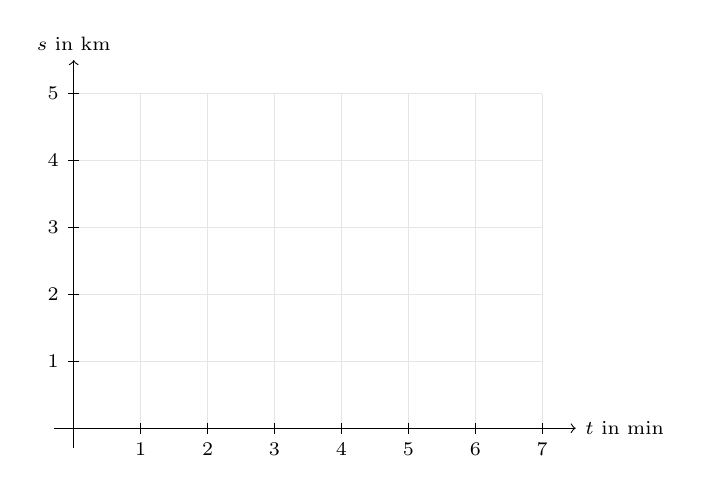
\begin{tikzpicture}[scale=0.85]
    \draw[gray!20] (0,0) grid (7,5);
    \draw[->] (-0.3,0) -- (7.5,0) node[right] {\scriptsize $t$ in min};
    \draw[->] (0,-0.3) -- (0,5.5) node[above] {\scriptsize $s$ in km};
    \foreach \x in {1,...,7} \draw (\x,0.08) -- (\x,-0.08) node[below] {\scriptsize \x};
    \foreach \y in {1,...,5} \draw (0.08,\y) -- (-0.08,\y) node[left] {\scriptsize \y};
  \end{tikzpicture}
  \end{center}
  \begin{solution}
  \begin{center}
  \begin{tikzpicture}[scale=0.85]
    \draw[gray!20] (0,0) grid (7,5);
    \draw[->] (-0.3,0) -- (7.5,0) node[right] {\scriptsize $t$ in min};
    \draw[->] (0,-0.3) -- (0,5.5) node[above] {\scriptsize $s$ in km};
    \foreach \x in {1,...,7} \draw (\x,0.08) -- (\x,-0.08) node[below] {\scriptsize \x};
    \foreach \y in {1,...,5} \draw (0.08,\y) -- (-0.08,\y) node[left] {\scriptsize \y};
    \draw[thick,titleblue] (0,0.6) -- (7,4.8);
    \draw[thick,accentorange] (0,0) -- (7,4.9);
    \filldraw[black] (6,4.2) circle (1.8pt);
  \end{tikzpicture}\\
  \footnotesize \textcolor{titleblue}{Hauptfeld} \quad \textcolor{accentorange}{Favorit}
  \end{center}
  \end{solution}

  \part[2] Lies aus deinem Diagramm ab: Nach welcher Zeit und bei welchem
  Ort holt der Favorit das Hauptfeld ein?
  \Antwortraum{2}
  \begin{solution}
  Die beiden Geraden schneiden sich bei etwa $t\approx\SI{6}{\minute}$,
  $s\approx\SI{4.2}{\kilo\meter}$.
  \end{solution}

  \part[2] Bestätige dein Ergebnis rechnerisch mithilfe der Gleichungen
  $s_H(t) = \SI{0.6}{\kilo\meter} + \SI{36}{\kilo\meter\per\hour}\cdot t$
  und $s_F(t) = \SI{42}{\kilo\meter\per\hour}\cdot t$.
  \Antwortraum{2}
  \begin{solution}
  Gleichsetzen:
  \[
    \SI{42}{\kilo\meter\per\hour}\cdot t = \SI{0.6}{\kilo\meter} + \SI{36}{\kilo\meter\per\hour}\cdot t
    \;\Rightarrow\;
    \SI{6}{\kilo\meter\per\hour}\cdot t = \SI{0.6}{\kilo\meter}
    \;\Rightarrow\;
    t = \SI{0.1}{\hour} = \SI{6}{\minute}.
  \]
  Eingesetzt: $s_F = \SI{42}{\kilo\meter\per\hour}\cdot\SI{0.1}{\hour} = \SI{4.2}{\kilo\meter}$.
  Das bestätigt die Ablesung aus dem Diagramm.
  \end{solution}
\end{parts}
\end{taskbox}
\end{questions}

\begin{questions}
\begin{taskbox}[Zusatzaufgabe: Zwei Züge treffen sich]
\question[6] Zwischen Jena und Naumburg ($\SI{45}{\kilo\meter}$
Entfernung) verkehren gleichzeitig zwei Züge in Gegenrichtung: Ein ICE
fährt von Naumburg Richtung Jena mit $\SI{130}{\kilo\meter\per\hour}$,
gleichzeitig startet von Jena ein Regionalexpress Richtung Naumburg mit
$\SI{90}{\kilo\meter\per\hour}$. Beide Bewegungen sind gleichförmig.

\begin{parts}
  \part[3] Zeichne die $s$-$t$-Diagramme beider Züge in dasselbe
  Diagramm. Wähle den Nullpunkt ($s=0$) in Naumburg.

  \begin{center}
  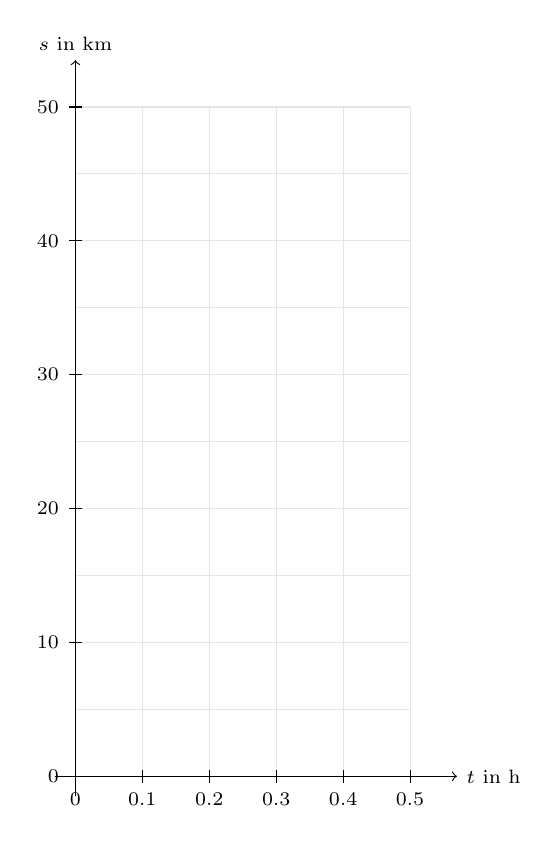
\begin{tikzpicture}[scale=0.85]
    \draw[gray!20] (0,0) grid[xstep=1,ystep=1] (5,10);
    \draw[->] (-0.3,0) -- (5.7,0) node[right] {\scriptsize $t$ in h};
    \draw[->] (0,-0.3) -- (0,10.7) node[above] {\scriptsize $s$ in km};
    \foreach \x/\lbl in {0/0,1/0.1,2/0.2,3/0.3,4/0.4,5/0.5} \draw (\x,0.1) -- (\x,-0.1) node[below] {\scriptsize \lbl};
    \foreach \y/\lbl in {0/0,2/10,4/20,6/30,8/40,10/50} \draw (0.1,\y) -- (-0.1,\y) node[left] {\scriptsize \lbl};
  \end{tikzpicture}
  \end{center}
  \begin{solution}
  \begin{center}
  \begin{tikzpicture}[scale=0.85]
    \draw[gray!20] (0,0) grid[xstep=1,ystep=1] (5,10);
    \draw[->] (-0.3,0) -- (5.7,0) node[right] {\scriptsize $t$ in h};
    \draw[->] (0,-0.3) -- (0,10.7) node[above] {\scriptsize $s$ in km};
    \foreach \x/\lbl in {0/0,1/0.1,2/0.2,3/0.3,4/0.4,5/0.5} \draw (\x,0.1) -- (\x,-0.1) node[below] {\scriptsize \lbl};
    \foreach \y/\lbl in {0/0,2/10,4/20,6/30,8/40,10/50} \draw (0.1,\y) -- (-0.1,\y) node[left] {\scriptsize \lbl};
    \draw[thick,titleblue] (0,0) -- (3.46,9) node[above right] {\scriptsize ICE};
    \draw[thick,accentorange] (0,9) -- (5,0);
    \node[accentorange,below right] at (3.7,2.34) {\scriptsize Regionalexpress};
    \filldraw[black] (2.05,5.32) circle (1.8pt);
  \end{tikzpicture}
  \end{center}
  \end{solution}

  \part[1] Bestimme aus deinem Diagramm möglichst genau, nach welcher Zeit
  und in welcher Entfernung von Naumburg sich die beiden Züge treffen.
  \Antwortraum{1}
  \begin{solution}
  Nach etwa $t\approx\SI{0.2}{\hour}$ ($\approx\SI{12}{\minute}$), in etwa
  $\SI{27}{\kilo\meter}$ Entfernung von Naumburg.
  \end{solution}

  \part[2] Bestätige dein Ergebnis rechnerisch.
  \Antwortraum{2}
  \begin{solution}
  Gleichungen für Ort und Zeit (Nullpunkt in Naumburg):
  $s_{ICE}(t) = \SI{130}{\kilo\meter\per\hour}\cdot t$,
  $s_{RE}(t) = \SI{45}{\kilo\meter} - \SI{90}{\kilo\meter\per\hour}\cdot t$.
  Gleichsetzen:
  \[
    \SI{130}{\kilo\meter\per\hour}\cdot t = \SI{45}{\kilo\meter} - \SI{90}{\kilo\meter\per\hour}\cdot t
    \;\Rightarrow\;
    \SI{220}{\kilo\meter\per\hour}\cdot t = \SI{45}{\kilo\meter}
    \;\Rightarrow\;
    t \approx \SI{0.205}{\hour} \approx \SI{12.3}{\minute}.
  \]
  Eingesetzt: $s_{ICE} = \SI{130}{\kilo\meter\per\hour}\cdot\SI{0.205}{\hour} \approx \SI{26.6}{\kilo\meter}$.
  Das bestätigt die Ablesung aus dem Diagramm.
  \end{solution}
\end{parts}
\end{taskbox}
\end{questions}

\end{document}
